%% Springer Nature journal submission.
%% To use the official class, replace the two lines below with
%%   \documentclass[sn-mathphys-num]{sn-jnl}
%% and remove the geometry/caption settings; the body requires no other change.
\documentclass[11pt]{article}

\usepackage[a4paper,margin=2.5cm]{geometry}
\usepackage{amsmath,amssymb}
\usepackage{graphicx}
\usepackage{booktabs}
\usepackage{multirow}
\usepackage{array}
\usepackage[numbers,sort&compress]{natbib}
\usepackage[font=small,labelfont=bf]{caption}
\usepackage{subcaption}
\usepackage{xcolor}
\usepackage{tikz}
\usetikzlibrary{arrows.meta,positioning,fit,backgrounds,calc}
\usepackage[colorlinks=true,allcolors=blue!60!black]{hyperref}
\usepackage[section]{placeins}   % floats may not drift past their section

% LaTeX defaults reserve most of a page for text, which makes a document with
% many full-width figures defer them all to the end. These allow a float to take
% more of a page and allow more floats per page, so each one stays near the text
% that refers to it.
\setcounter{topnumber}{3}
\setcounter{bottomnumber}{2}
\setcounter{totalnumber}{5}
\renewcommand{\topfraction}{0.9}
\renewcommand{\bottomfraction}{0.7}
\renewcommand{\textfraction}{0.07}
\renewcommand{\floatpagefraction}{0.7}

\newcommand{\aucm}{\text{AUC}}
\newcommand{\pmstd}[2]{$#1_{\pm#2}$}

\title{\bfseries Adaptive Sparse Temporal Attention and Evaluation Reliability
in Weakly-Supervised Video Anomaly Detection}

\author{}
\date{}

\begin{document}
\maketitle

\begin{abstract}
Weakly-supervised video anomaly detection assigns frame-level anomaly scores
from video-level labels. We study the problem on UCF-Crime along two axes.
First, we introduce ATA-HS, a detector combining multi-scale dilated temporal
convolution with $\alpha$-entmax sparse temporal attention whose sparsity level
is predicted per video, and a hybrid score that fuses a multiple-instance term,
a deviation-from-normal term and a temporal prediction term through an
input-conditioned gate. Sparse attention with exact zeros is differentiable,
unlike hard top-$K$ selection, so the temporal selector is trained by the task
loss. Second, we quantify the reliability of the benchmark itself by
bootstrapping over videos rather than frames, the level at which the data are
independent. Over five seeds the full model reaches $0.766_{\pm0.014}$ frame-level
AUC against $0.778_{\pm0.004}$ for a multiple-instance baseline, a difference a
paired video-level bootstrap does not resolve, while attaining higher average
precision ($0.204$ against $0.189$, base rate $0.076$) and lowering the
false-alarm rate at the conventional fixed threshold from $0.022$ to $0.016$. That
last advantage does not survive scrutiny: measured at a matched detection rate,
which is invariant to the scale of a model's outputs, the ordering reverses, and
the model with by far the worst fixed-threshold false-alarm rate has the best
threshold-free one. The video-level bootstrap gives a $95\%$ confidence
interval of $\pm7.6$ AUC points on a single test estimate, an order of magnitude
larger than the one- to two-point differences commonly reported between methods. We
further show that validation video-level AUC does not predict test frame-level
AUC ($r=-0.37$, $n=18$), and that frame-level AUC of $0.77$ coexists with a
median temporal localisation IoU of $0.00$. Code, trained model and a deployed
application are released.

\smallskip
\noindent\textbf{Keywords:} video anomaly detection, weak supervision,
sparse attention, evaluation methodology, surveillance
\end{abstract}

\section{Introduction}
\label{sec:intro}

Closed-circuit television is the dominant technical response to crime in public
space, and installed capacity has grown to the order of one billion cameras
worldwide. Whether that capacity prevents crime depends on how the footage is
used. A systematic review of $76$ CCTV interventions spanning four decades finds
an overall reduction in crime that is statistically significant but
modest, and concentrated in schemes where footage is actively
monitored rather than only recorded~\citep{piza2019cctv}. The constraint is
therefore not the number of cameras but the number of feeds a person can watch.

That constraint is a property of human attention rather than of training or
staffing levels. Operators monitoring several feeds miss a substantial fraction
of staged target events, and the miss rate rises as the number of concurrent
views increases~\citep{sulman2008effective}; the finding that sustained attention
to an uneventful feed degrades within tens of minutes has been reported in the
security-technology literature for
decades~\citep{green1999appropriate}. Display parameters compound the
problem, since reducing frame rate below a threshold measurably lowers detection
performance in controlled tasks~\citep{keval2008cctv}. A control room with more
cameras than operators consequently produces evidence for retrospective
investigation, but does not produce detection early enough to intervene.

Automation is directed at this review bottleneck rather than at recording
capacity. If a system can rank time intervals by how unusual they are, an
operator need only inspect the highest-ranked fraction of the footage, and the
effective number of feeds one person can supervise increases. The difficulty is
that the events of interest are defined by their absence from what is normal.
They are rare, heterogeneous, and cannot be enumerated in advance, so the task
resists formulation as closed-set
classification~\citep{dee2008how,ramachandra2020survey,nayak2021comprehensive}: a
detector trained on a fixed inventory of event types must still respond to an
event outside it. This is why the field models normality and measures departure
from it, rather than learning one class per crime.

Modelling normality requires knowing which footage is normal, and annotating
surveillance archives frame by frame is not feasible at the scale at which they
accumulate. The compromise that has become standard is weak supervision. Training
uses a single binary label per video, recording only that an anomalous event
occurs somewhere within it and never where; evaluation is nevertheless at frame
level, because that is what an operator needs~\citep{sultani2018real}. The
learning problem is therefore to recover temporal localisation that was never
supervised. UCF-Crime, introduced alongside this formulation, contains $1900$
untrimmed real-world surveillance videos across $13$ anomaly categories and
remains the standard benchmark for the setting.

Two properties of that benchmark, shown in Figure~\ref{fig:dataset}, shape both
what a model must do and what an experiment can establish. The category balance
differs between the splits: Robbery contributes $145$ training videos and $5$
test videos, while Shooting contributes $27$ and $23$, so the categories a model
sees most during training are among the least represented when it is scored.
Events are also short relative to the videos containing them. The annotated
interval occupies a median $14\%$ of its video and the positive frame rate over
the test set is $7.6\%$, while mean event duration ranges from $3$\,s for Abuse
and RoadAccidents to $95$\,s for Assault. No single temporal scale is adequate,
and any bag-level aggregation that averages over too many snippets will dilute a
short event into its surrounding context.

\begin{figure}[htbp]
\centering
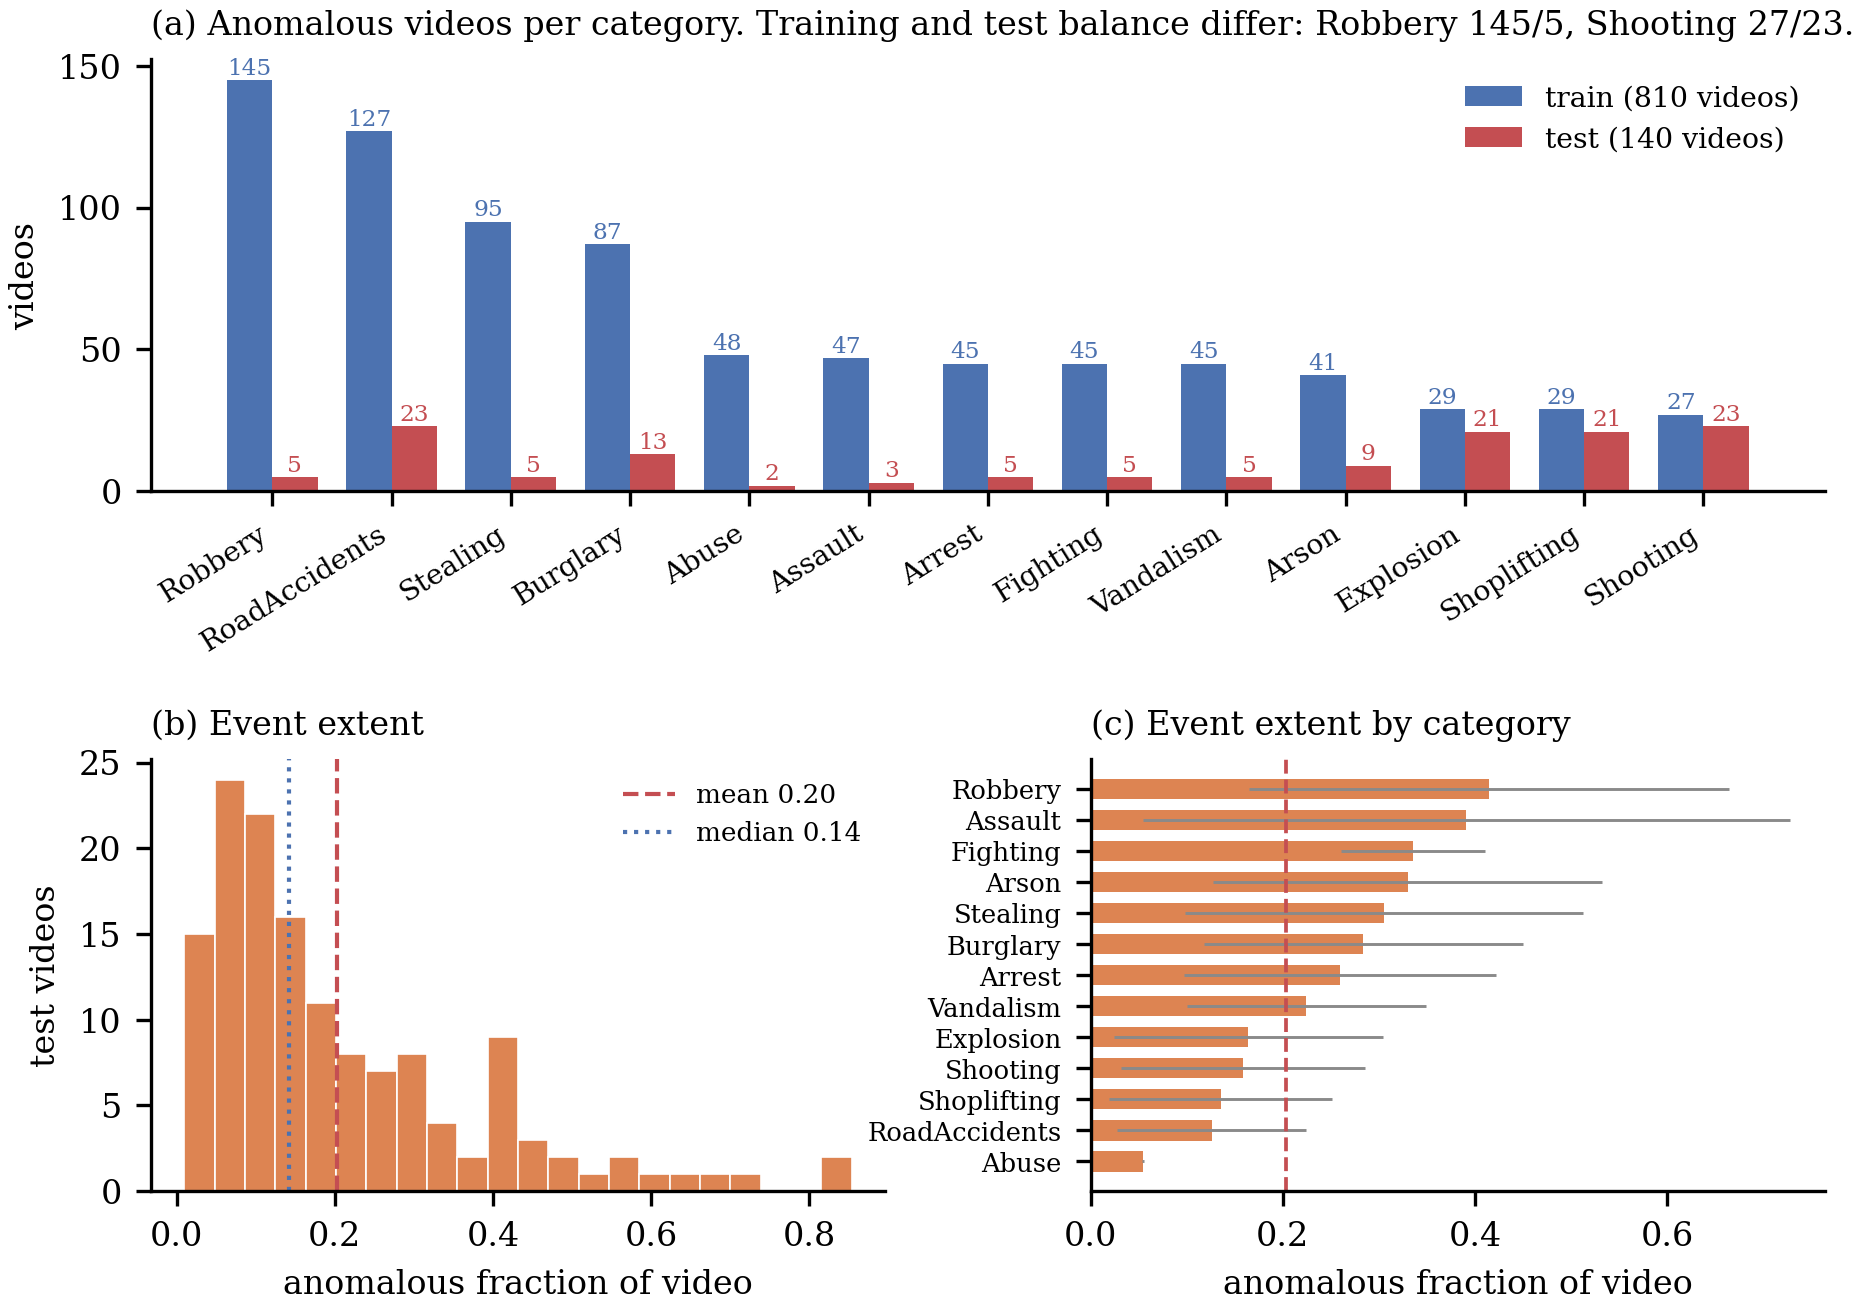
\includegraphics[width=\linewidth]{figures/fig_dataset.png}
\caption{UCF-Crime composition. (a) Anomalous videos per category in each split.
The training and test balances differ substantially: the categories most
represented in training are among the least represented at test time. (b)
Fraction of each test video occupied by the annotated event; the median is
$0.14$. (c) The same quantity per category, with standard deviation.}
\label{fig:dataset}
\end{figure}

Against this benchmark, reported frame-level AUC has risen from
$75.4$~\citep{sultani2018real} to $88.0$~\citep{wu2024vadclip}. The increments
are typically one to two points per publication, and are ordinarily obtained from
a single training run reported without an uncertainty estimate. The test set
comprises $290$ videos, and frames within a video are strongly correlated, so the
effective sample size is closer to the number of videos than to the million
frames they contain. Whether an increment of one or two points is distinguishable
from run-to-run and sampling variation on a test set of that size has not, to our
knowledge, been established. This question is logically prior to comparing
methods, because it determines what a comparison can demonstrate.

We address both the modelling problem and the measurement one.

We make three contributions.

\textbf{Frame-level AUC does not measure temporal localisation.} A mean-pooling
model that emits one score per video, and therefore cannot localise at all,
reaches $0.775$ frame-level AUC on UCF-Crime, statistically indistinguishable
from every detector we test including the multiple-instance baseline at $0.778$.
A detector near $0.77$ AUC has a median temporal intersection-over-union of
$0.000$ against the annotated intervals, exceeding $0.5$ on $5$ of $140$
anomalous videos. The measure the benchmark is ordinarily compared on largely
answers whether a video contains an anomaly, not where it is.

\textbf{Reported differences are small relative to measurement variability.}
Resampling test videos rather than frames, the unit at which the data are
independent, gives a $95\%$ interval of $\pm7.6$ AUC points on a single estimate.
Across seeds, architectures vary by up to $0.04$ AUC, and the ranking of ablations
reverses between three seeds and five. Both are an order of magnitude larger than
the one- to two-point differences commonly reported between methods.

\textbf{A learned sparsity budget for temporal selection.} ATA-HS selects
snippets with $\alpha$-entmax~\citep{peters2019sparse}, which assigns exactly
zero weight outside the selected set while remaining differentiable; hard top-$K$
is piecewise constant in the selection scores and propagates no gradient to the
selector. A gate predicts the entmax temperature rather than fixing it. Under a
controlled comparison this attains higher accuracy and lower seed variance than
dense attention, than entmax at a fixed temperature, and than non-differentiable
top-$K$. We show by direct measurement that the gate does not adapt to event
duration as we first supposed, but supplies a sparsity schedule during training
that a hand-set constant does not reproduce.

The architectural result is not an accuracy improvement: ATA-HS reaches
$0.766_{\pm0.014}$ AUC against $0.778_{\pm0.004}$ for the baseline, a difference
a paired bootstrap does not resolve. It is ahead on average precision
($0.204$ against $0.189$) and lowers the false-alarm rate at threshold $0.5$ from
$0.022$ to $0.016$, though that last advantage proves to be a property of the
score scale: measured at a matched detection rate it disappears and reverses.
We report the comparison this way because the measurement
analysis above applies to our own claims as much as to the published increments
against which they would be compared.

\section{Related work}
\label{sec:related}

\subsection{One-class formulations}
Early VAD methods train only on normal video and treat reconstruction or
prediction error as an anomaly score. Convolutional autoencoders model
appearance and short-range motion~\citep{hasan2016learning}; future-frame
prediction with an adversarial objective improves temporal
sensitivity~\citep{liu2018future}. Because autoencoders generalise to unseen
inputs, memory modules restrict reconstruction to a learned dictionary of normal
patterns~\citep{gong2019memorizing}, and prototype memories combined with frame
prediction refine this further~\citep{park2020learning}. Sparse-coding
formulations pursue the same
objective with an explicit dictionary~\citep{lu2013abnormal,luo2017revisit}.
These methods are effective on constrained scenes such as
UCSD~\citep{mahadevan2010anomaly}, where anomalies are largely motion
irregularities, but transfer poorly to unconstrained footage in which normal
appearance is itself highly variable.

\subsection{Weakly-supervised formulations}
\citet{sultani2018real} introduced UCF-Crime and cast the task as multiple-instance
learning: each video is a bag of $32$ temporal segments, and a ranking loss
separates the highest-scoring segment of an anomalous bag from that of a normal
bag, with sparsity and smoothness regularisers. Subsequent work improves the
instance-selection signal. \citet{zhong2019graph} treat weak labels as noisy
frame labels cleaned by a graph convolutional network. RTFM~\citep{tian2021weakly}
observes that feature magnitude separates abnormal from normal snippets and
selects instances by magnitude with a multi-scale temporal network.
MSL~\citep{li2022self} replaces single-instance selection with sequence
selection; S3R~\citep{wu2022self} adds a dictionary-based reconstruction term;
UR-DMU~\citep{zhou2023dual} maintains separate normal and abnormal memories with
uncertainty regulation; MGFN~\citep{chen2023mgfn} contrasts glance and focus
representations. Reported frame-level AUC on UCF-Crime rises across this line of
work from $75.41$ for the original multiple-instance
formulation~\citep{sultani2018real} to $82.12$~\citep{zhong2019graph},
$84.30$~\citep{tian2021weakly}, $85.30$~\citep{li2022self},
$85.99$~\citep{wu2022self}, and $86.97$--$86.98$ for the memory- and
contrast-based variants~\citep{zhou2023dual,chen2023mgfn}. A parallel line removes labels entirely: generative cooperative
learning trains a generator and discriminator jointly on unlabelled video and
reaches accuracy between the one-class and weakly-supervised
regimes~\citep{zaheer2022generative}.

\subsection{Deep feature representations for video}
The representation on which a detector operates has driven much of the reported
progress, independently of the detection head. Early deep VAD systems consumed
raw frames or stacked optical flow through 2-D convolutional autoencoders, which
capture appearance but model motion only over the few frames in the input
stack~\citep{hasan2016learning}. C3D~\citep{tran2015learning} replaced this with
learned 3-D convolution over $16$-frame clips and supplied the features for the
original UCF-Crime baseline. I3D~\citep{carreira2017quo} inflated 2-D ImageNet
kernels into 3-D and pretrained on Kinetics, yielding clip descriptors that
transfer markedly better; it remains the standard input for weakly-supervised
detectors, and the $16$-frame snippet it induces has become the de facto temporal
unit of the task. Alternatives differ in how they allocate capacity between
appearance and motion: TSN~\citep{wang2016temporal} samples sparse segments across
the whole video, SlowFast~\citep{feichtenhofer2019slowfast} runs two pathways at
different frame rates, and Video Swin~\citep{liu2022video} applies shifted-window
self-attention over space-time. Two-stream variants that add explicit flow, or
motion-aware distillation of flow into an appearance
network~\citep{zhu2019motion}, improve sensitivity to velocity anomalies at
additional extraction cost. Most recently, image-text pretraining has displaced
action-recognition pretraining: CLIP~\citep{radford2021learning} embeddings carry
semantic information absent from Kinetics features, and substituting them raises
reported UCF-Crime AUC by several points without altering the detection
head~\citep{joo2023clip,wu2024vadclip}. Because backbone and head are usually
changed together, the attribution of reported gains between the two is often
ambiguous; we therefore hold the backbone fixed across all configurations in
Section~\ref{sec:experiments}.

\subsection{Temporal modelling architectures}
Given snippet features, detectors differ in how they aggregate them over time.
The original multiple-instance formulation scores each of $32$ segments
independently with a small multilayer perceptron, so no information crosses
segment boundaries and the model is invariant to their order~\citep{sultani2018real};
temporal continuity enters only as a smoothness penalty on the output. Recurrent
formulations model the sequence explicitly, with convolutional
LSTMs~\citep{shi2015convolutional} propagating a spatial hidden state across
frames for reconstruction-based detection~\citep{luo2017remembering}, though
recurrence over long untrimmed footage is expensive and gradients attenuate over
the thousands of snippets a surveillance video can contain. Temporal convolution
avoids recurrence: RTFM~\citep{tian2021weakly} applies a pyramid of dilated
convolutions so each snippet sees several seconds of context at fixed cost, a
design we adopt in Section~\ref{sec:method}. Graph formulations treat snippets as
nodes with feature-similarity or temporal-adjacency edges, which allows
non-adjacent but visually similar snippets to exchange
information~\citep{zhong2019graph}. Self-attention~\citep{vaswani2017attention}
generalises this to learned, content-dependent connectivity and now dominates:
it has been combined with conditional random fields to enforce temporal
consistency~\citep{purwanto2021dance}, applied over CLIP features with temporal
self-attention~\citep{joo2023clip}, and paired with self-training to refine
snippet-level pseudo-labels~\citep{feng2021mist,lv2021localizing}. Attention is
also used for selection rather than aggregation, retaining the highest-scoring
snippets and discarding the remainder; the selection is normally a hard top-$K$
operation, which is not differentiable with respect to the selection scores. Our
model differs in this respect, replacing hard selection with an exactly sparse
but differentiable transformation whose sparsity level is predicted per video.

\subsection{Vision-language and training-free formulations}
Replacing action-recognition features with CLIP embeddings raises reported
accuracy: CLIP-TSA~\citep{joo2023clip} applies temporal self-attention over CLIP
features, and VadCLIP~\citep{wu2024vadclip} adapts the vision-language alignment
directly. LAVAD~\citep{zanella2024harnessing} scores anomalies without training
by captioning frames and querying a language model. The reported figures are
$87.58$ and $88.02$ respectively for the two CLIP-based
detectors~\citep{joo2023clip,wu2024vadclip}, obtained without altering the
detection head, so the gain over the I3D-based systems above is attributable to
the representation rather than to the detector. Across the whole line of work the
backbone changes from C3D to TSN to I3D to CLIP while the reported range spans
$75.4$ to $88.0$; the two are not separable from the published numbers alone. We
return to this in Section~\ref{sec:discussion}, where the measured confidence
interval on this test set is $\pm7.6$ points. Self-supervised multi-task
formulations~\citep{georgescu2021anomaly} occupy an intermediate position.

\subsection{Sparse attention}
Softmax attention assigns non-zero weight to every position. Sparsemax
projects onto the simplex, producing exact zeros~\citep{martins2016softmax};
$\alpha$-entmax interpolates between the two, with $\alpha=1.5$ admitting an
exact sorting-based solution and a defined Jacobian~\citep{peters2019sparse}.
This is the property we require: hard top-$K$ selection is not differentiable
with respect to the selection scores, so a selector trained through it receives
no gradient.

\subsection{Evaluation methodology}
Variance-aware benchmarking is established in adjacent
fields~\citep{reimers2017reporting,bouthillier2021accounting} but is not standard
in VAD, where single-run numbers without intervals are the norm. Region- and
track-based criteria have been proposed to expose localisation quality that
frame-level AUC hides~\citep{ramachandra2020street}. \citet{delong1988comparing}
give a variance estimator for correlated AUCs, though its independence assumption
is violated by frames drawn from the same video.

\section{Method}
\label{sec:method}

\subsection{Problem formulation}
A video is divided into $T$ non-overlapping snippets of $16$ frames. A frozen
backbone maps snippet $t$ to $\mathbf{x}_t \in \mathbb{R}^{D}$, giving
$X = [\mathbf{x}_1,\dots,\mathbf{x}_T]$. Training provides a single label
$y \in \{0,1\}$ per video. The model outputs per-snippet scores
$\mathbf{s} \in [0,1]^{T}$, expanded to frame level for evaluation.

\subsection{Adaptive sparse temporal attention}

\paragraph{Multi-scale temporal context.}
Snippet features are projected to $d$ dimensions and passed through four
parallel dilated convolutions with dilation rates $\{1,2,4,8\}$ and kernel size
$3$, concatenated and added residually. Receptive fields span $3$ to $17$
snippets, that is $1.6$ to $9.1$ seconds at $30$ fps, covering the duration of
the events annotated in UCF-Crime (Figure~\ref{fig:mech}a). Padded positions are masked before and after
convolution so that a dilated kernel straddling the boundary cannot mix padding
into real positions.

\paragraph{Sparse attention with a predicted budget.}
Let $H = [\mathbf{h}_1,\dots,\mathbf{h}_T]$ denote the contextualised features.
A scoring network produces logits $z_t = w^{\top}\tanh(W\mathbf{h}_t)$. A gate
reads the masked mean $\bar{\mathbf{h}}$ and predicts a temperature
\begin{equation}
\tau = \exp\!\big(\beta \tanh(g(\bar{\mathbf{h}}))\big), \qquad \beta = 1.5,
\label{eq:temp}
\end{equation}
bounding $\tau \in (e^{-\beta}, e^{\beta})$. Attention weights are
\begin{equation}
\boldsymbol{\alpha} = \operatorname{entmax}_{1.5}(\mathbf{z}/\tau),
\label{eq:entmax}
\end{equation}
where $\operatorname{entmax}_{1.5}(\mathbf{z})_t = [\,\mathbf{z}_t/2 - \tau^{*}\,]_{+}^{2}$
with threshold $\tau^{*}$ obtained by sorting~\citep{peters2019sparse}. Weights
below the threshold are exactly zero, so the realised support size is a learned,
input-dependent quantity rather than a fixed $K$ (Figure~\ref{fig:mech}b,c). Padded positions are masked
with a large finite negative value; $-\infty$ produces $\infty-\infty$ in the
variance term of the closed-form solution. The threshold argument is clamped
away from zero before the square root, since $\mathrm{d}\sqrt{x}/\mathrm{d}x$ is
unbounded at $x=0$ and yields NaN gradients when a coordinate lies on the
support boundary.


\begin{figure}[htbp]
\centering
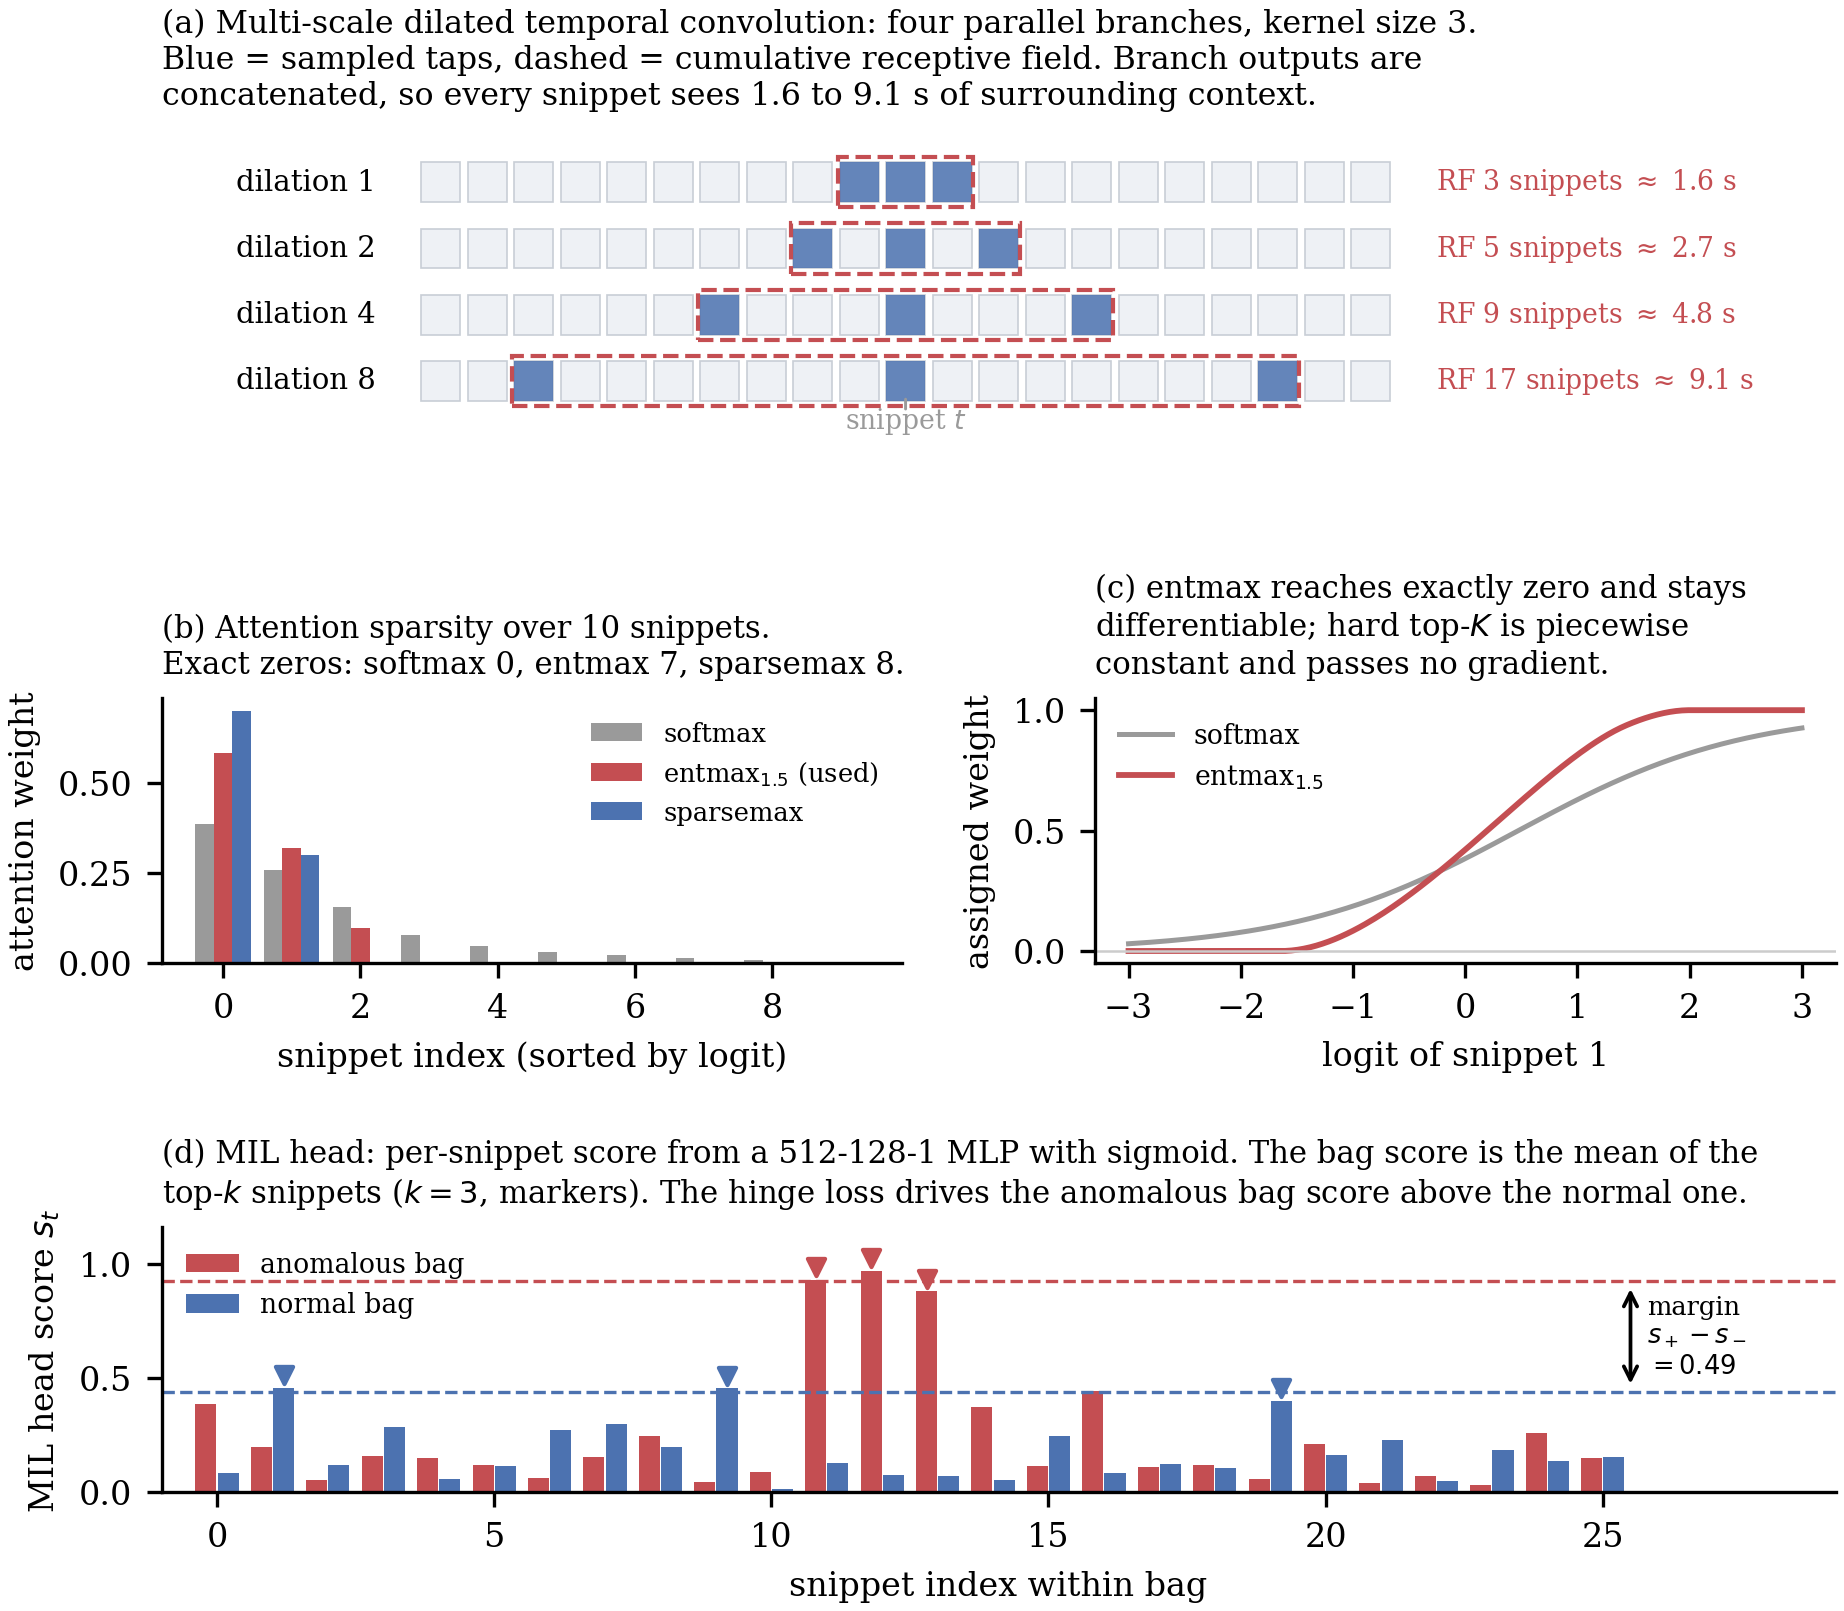
\includegraphics[width=\linewidth]{figures/fig_mechanisms.png}
\caption{Components of ATA-HS. (a) Four dilated convolution branches, kernel size
three. Blue marks the sampled taps and the dashed box the cumulative receptive
field, which spans $1.6$ to $9.1$\,s once the branch outputs are concatenated.
(b) Attention weights over ten snippets: softmax assigns non-zero weight
everywhere, entmax$_{1.5}$ produces seven exact zeros, sparsemax eight.
(c) Weight assigned to one snippet as its logit varies. entmax reaches exactly
zero and remains differentiable, whereas hard top-$K$ selection is piecewise
constant and propagates no gradient to the selector. (d) The multiple-instance
head. Per-snippet scores come from a $512\!-\!128\!-\!1$ network; the bag score is
the mean of the top $k$ (markers, $k=3$), and the hinge loss separates the
anomalous bag score from the normal one.}
\label{fig:mech}
\end{figure}

\subsection{Hybrid scoring}
Three heads produce per-snippet scores. The multiple-instance head applies an MLP
followed by a sigmoid. The deviation head measures distance from a learned normal
centre $\mathbf{c}$, $s^{\mathrm{mag}}_t = \sigma(\gamma(\|\mathbf{h}_t-\mathbf{c}\|-\mu))$,
where $\mu$ is the mean over unpadded positions. The temporal head predicts
$\mathbf{h}_{t+1}$ from $\mathbf{h}_t$ and uses the residual norm, centred the
same way. A gate emits per-snippet mixing weights
$\mathbf{w}_t = \operatorname{softmax}(g_f(\mathbf{h}_t))$ and the final score is
$s_t = \sum_i w_{t,i}\, s^{(i)}_t$.

The centring statistics must be computed over unpadded positions only. Training
batches contain substantial padding while inference processes one unpadded video,
so an unmasked mean makes a snippet's score depend on the padding present in its
batch. Section~\ref{sec:results} quantifies the cost of this error.

\subsection{Objective}
The bag score is the mean of the top-$k$ snippet scores. With a positive frame
rate of $7.6\%$, a proportional $k$ over-selects; we use a small absolute $k$.
The objective combines a ranking hinge over anomalous--normal bag pairs with
smoothness and sparsity terms on anomalous bags and an entropy term on the
attention distribution,
\begin{equation}
\mathcal{L} = \underbrace{\big[1 - s^{\mathrm{bag}}_{+} + s^{\mathrm{bag}}_{-}\big]_{+}}_{\text{ranking}}
 + \lambda_{1}\!\sum_t (s_{t+1}-s_t)^2
 + \lambda_{2}\!\sum_t s_t
 + \lambda_{3}\, \mathcal{H}(\boldsymbol{\alpha}),
\label{eq:loss}
\end{equation}
where $\mathcal{H}$ is the entropy of the attention weights. Penalising
$\mathcal{H}$ makes the gate pay for every snippet it retains, so the support
stays small unless the content requires otherwise.

\begin{figure}[htbp]
\centering
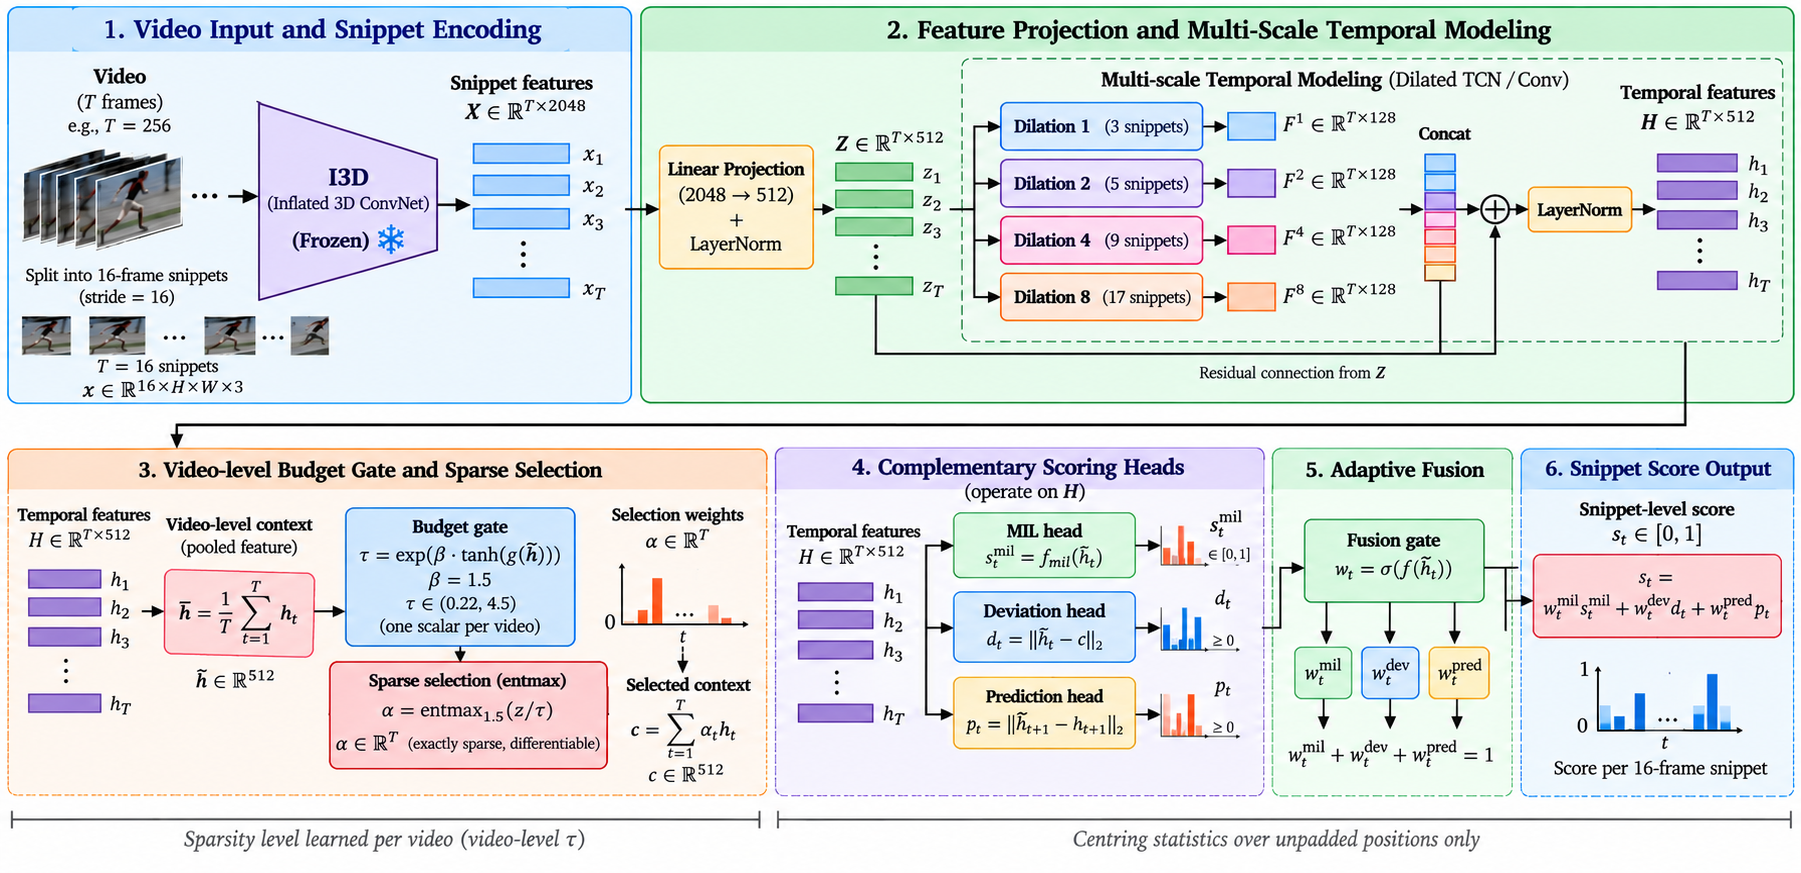
\includegraphics[width=\linewidth]{figures/fig_architecture.png}
\caption{ATA-HS. (1) A frozen I3D backbone encodes non-overlapping $16$-frame
snippets into $\mathbf{x}_t\in\mathbb{R}^{2048}$. (2) Features are projected to
$512$ dimensions and passed through four dilated temporal convolutions with rates
$\{1,2,4,8\}$, giving receptive fields of $3$ to $17$ snippets. (3) A budget gate
predicts the attention temperature, and $\alpha$-entmax converts the scores into
exactly sparse selection weights $\boldsymbol{\alpha}$. (4) Three heads score each
snippet: a supervised multiple-instance term, a deviation from a learned normal
centre, and a next-snippet prediction error. (5) A fusion gate emits per-snippet
mixing weights summing to one. (6) The output is a score $s_t\in[0,1]$ per
snippet, expanded to frame level for evaluation.}
\label{fig:arch}
\end{figure}

\section{Evaluation protocol}
\label{sec:protocol}

\subsection{Dataset}
UCF-Crime~\citep{sultani2018real} contains $1900$ untrimmed surveillance videos
across $13$ anomaly categories. The official split is $1610$ training videos
($810$ anomalous, $800$ normal) with video-level labels and $290$ test videos
($140$ anomalous, $150$ normal) with frame-level temporal annotation. We verified
our copy of the split and annotation files against the authors' release: the
files are identical, and the resulting frame counts are $1{,}111{,}808$ with a
positive rate of $0.0759$.

\subsection{Metrics}
The protocol concatenates all frames of all $290$ test videos into a single ROC;
we denote this micro AUC and report it as the primary metric. We additionally
report: macro AUC, the mean of per-video AUC, defined only for the $140$
anomalous videos; $\aucm_{\mathrm{A}}$, computed over anomalous videos only,
which isolates localisation from the ability to remain silent on normal video;
the false-alarm rate on normal videos at threshold $0.5$; and average precision
with its base rate, since a constant predictor attains AP equal to the base rate.

\subsection{Reliability estimation}
Frames within a video are strongly correlated, so resampling frames understates
uncertainty. We resample whole videos with replacement ($2000$ iterations) and
report the percentile interval~\citep{efron1986bootstrap}. Method comparisons use a paired video-level
bootstrap over the same resampled videos. We report DeLong intervals only for
reference; its independence assumption does not hold here.

\section{Experiments}
\label{sec:experiments}

\subsection{Implementation}
Snippet features are extracted with I3D-ResNet50 pretrained on
Kinetics-400~\citep{carreira2017quo} at $224\times224$ centre crop, giving
$D=2048$. Most published UCF-Crime results use I3D-Inception with $D=1024$;
because we extract training and test features with the same backbone, our
results are internally consistent, and our baseline reproduction should be
compared against the published range rather than to $75.41$ exactly. ATA-HS uses
$d=512$, dropout $0.3$, Adam at $10^{-3}$, $40$ epochs, batches of $32$ bags with
equal anomalous and normal counts. The baseline is the multiple-instance
model of \citet{sultani2018real} with $32$ segments. Checkpoints are selected on a
validation split held out from the \emph{training} videos; the test set is used
once, to produce the reported numbers.

\subsection{Baseline reproduction}
The multiple-instance baseline attains $0.7792$ micro AUC with a false-alarm rate
of $0.0228$, against the published $0.7541$ and $0.019$ obtained with C3D
features. The difference is consistent with the change of backbone. We treat this
as evidence that the pipeline and the harness reproduce the reference behaviour.

\section{Results}
\label{sec:results}

\subsection{Detection accuracy and false alarms}

\begin{table}[htbp]
\centering
\caption{ATA-HS ablation on the UCF-Crime test set. Mean $\pm$ standard deviation; $n$ is the number of seeds. AP is reported with the test-set positive rate of $0.0759$, against which a constant predictor scores $0.076$. $\aucm_{\mathrm{A}}$ is restricted to the $140$ anomalous videos. No AUC value is marked best, since the sampling uncertainty of a single estimate on this test set exceeds the differences between rows.}
\label{tab:main}
\small
\begin{tabular}{lcccccc}
\toprule
Model & $n$ & AUC & AP & $\aucm_{\mathrm{A}}$ & FAR$_{0.5}$ & $\Delta$FAR \\
\midrule
ATA-HS (full) & 5 & $0.766_{\pm0.014}$ & $0.204_{\pm0.004}$ & $0.585_{\pm0.008}$ & $0.016_{\pm0.003}$ & $-26\%$ \\
MIL baseline \citep{sultani2018real} & 5 & $0.778_{\pm0.004}$ & $0.189_{\pm0.005}$ & $0.580_{\pm0.006}$ & $0.022_{\pm0.003}$ & --- \\
\midrule
\quad $-$ entmax (softmax) & 5 & $0.760_{\pm0.038}$ & $\mathbf{0.210}_{\pm0.015}$ & $\mathbf{0.597}_{\pm0.018}$ & $0.015_{\pm0.005}$ & $-33\%$ \\
\quad $-$ adaptive budget & 5 & $0.723_{\pm0.034}$ & $0.195_{\pm0.017}$ & $0.568_{\pm0.015}$ & $\mathbf{0.011}_{\pm0.005}$ & $-50\%$ \\
\quad $-$ hybrid heads & 3 & $0.764_{\pm0.013}$ & $0.175_{\pm0.003}$ & $0.573_{\pm0.012}$ & $0.012_{\pm0.002}$ & $-47\%$ \\
\quad $-$ multi-scale & 3 & $0.755_{\pm0.024}$ & $0.206_{\pm0.014}$ & $0.588_{\pm0.016}$ & $0.011_{\pm0.005}$ & $-47\%$ \\
\bottomrule
\end{tabular}
\end{table}


Table~\ref{tab:main} and Figure~\ref{fig:ablation} report the main result.
ATA-HS matches the baseline in detection accuracy and separates from it in false
alarms.

On AUC the two are not distinguishable. The best ATA-HS configuration
reaches $0.766_{\pm0.014}$ against $0.778_{\pm0.004}$ for the baseline, a
difference of $0.012$. The
$95\%$ video-level bootstrap interval for this test set has a half-width of
$0.076$, so the observed difference is $7\%$ of the interval and the paired
bootstrap does not separate the two methods. Reporting either as superior on this
evidence would not be supportable.

On average precision and on the false-alarm rate at threshold $0.5$ the two do
separate. The full model scores $0.204$ AP against $0.189$, above the $0.076$ base
rate for both, and $0.016_{\pm0.004}$ FAR against the baseline's
$0.022_{\pm0.004}$. The false-alarm effect is not confined to one configuration:
all five ATA-HS variants in Table~\ref{tab:main} sit below the baseline, by
between $24\%$ and $50\%$, surviving the removal of the multi-scale branch, the
hybrid heads, the adaptive budget and entmax individually. The largest reduction
is $50\%$, to $0.011_{\pm0.005}$, without the multi-scale branch.
Section~\ref{sec:threshold} then measures the same quantity without a fixed
threshold and finds the ordering does not hold, so the FAR$_{0.5}$ column should
be read as a statement about the models' output scales. Average precision, which
is threshold-free, is not subject to that objection.

\begin{figure}[htbp]
\centering
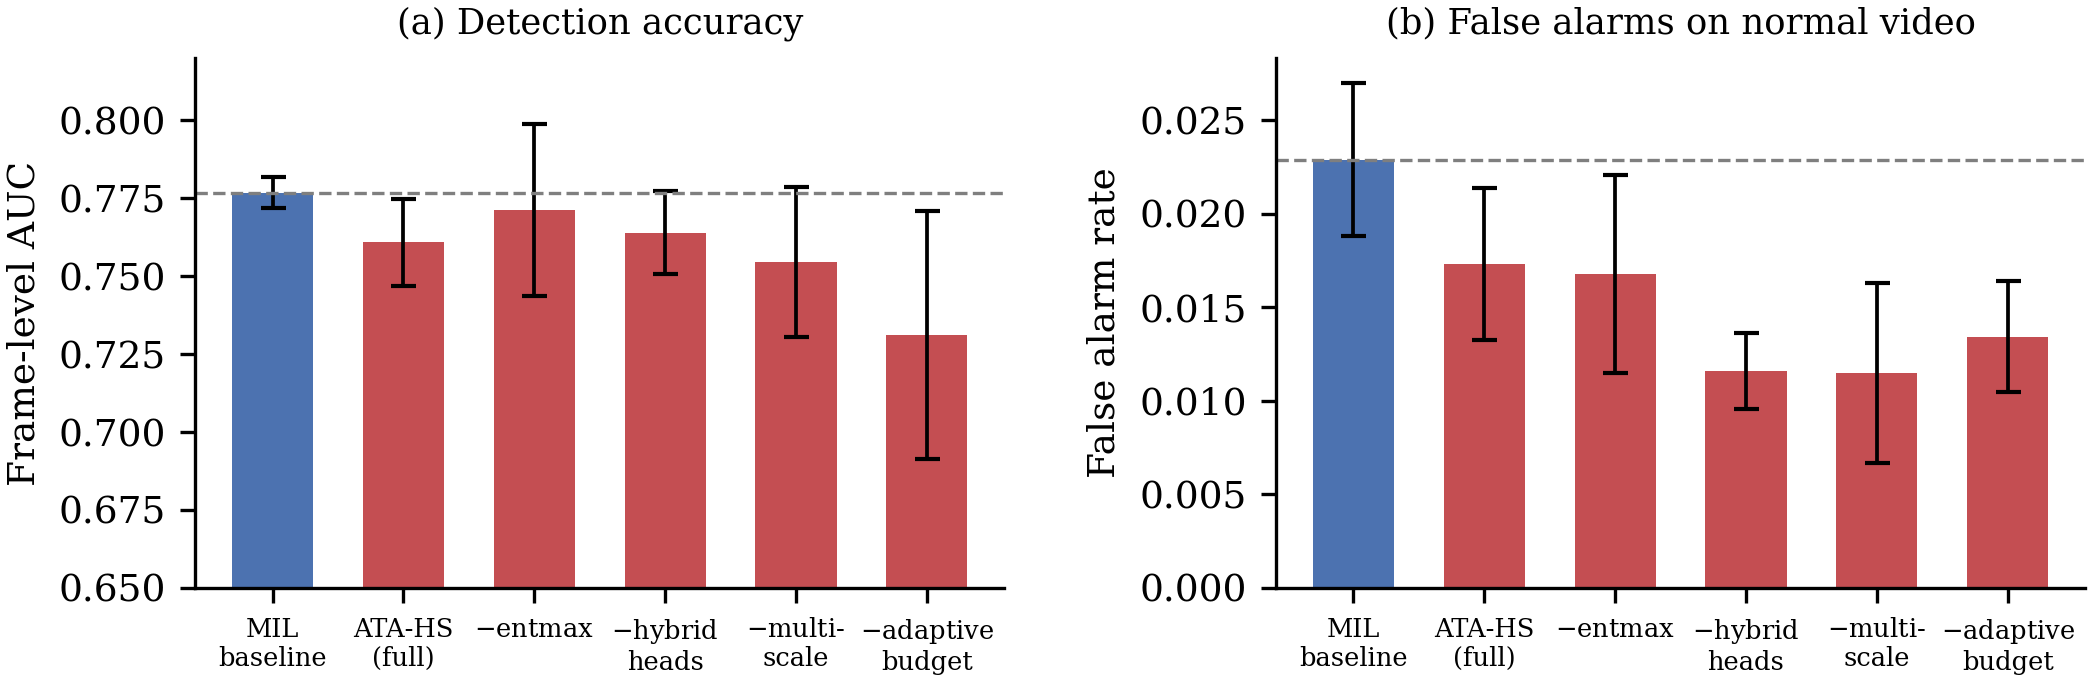
\includegraphics[width=\linewidth]{figures/fig_ablation.png}
\caption{Component ablation. Dashed line marks the baseline. No configuration
separates from the baseline in AUC; all sit below it on the fixed-threshold
false-alarm rate, an effect Section~\ref{sec:threshold} attributes to score scale.}
\label{fig:ablation}
\end{figure}

\begin{table}[htbp]
\centering
\caption{Controlled comparison on the UCF-Crime test set. Every method consumes the same I3D features, the same official split and the same three seeds, so rows differ only in the model. AUC is frame-level over all $290$ test videos; $\aucm_{\mathrm{A}}$ is restricted to the $140$ anomalous videos and therefore reflects localisation; FAR is measured on normal videos at threshold $0.5$, with $\Delta$FAR its change relative to the multiple-instance baseline. $p$ is a paired video-level bootstrap of the AUC difference against the proposed model. Mean $\pm$ standard deviation over three seeds. No AUC value is marked best: every $p$ exceeds $0.16$, so no pair of methods is separated on that measure. Best values are marked in the two columns that do separate them; note that the FAR$_{0.5}$ column is measured at a fixed threshold and so reflects the scale of each model's scores as well as its detection, which Table~\ref{tab:threshold} separates. Mean pooling emits one score per video and cannot localise; it is included to show how much frame-level AUC is attainable without localisation.}
\label{tab:comparison}
\small
\begin{tabular}{lcccccc}
\toprule
Method & AUC & $p$ & $\aucm_{\mathrm{A}}$ & FAR$_{0.5}$ & $\Delta$FAR & Params (M) \\
\midrule
\textbf{ATA-HS (proposed)} & $0.761_{\pm0.014}$ & --- & $\mathbf{0.582}_{\pm0.009}$ & $\mathbf{0.017}_{\pm0.004}$ & $-24\%$ & 2.66 \\
\midrule
MIL ranking \citep{sultani2018real} & $0.777_{\pm0.005}$ & $0.74$ & $0.580_{\pm0.009}$ & $0.023_{\pm0.004}$ & --- & 1.07 \\
Dense self-attention & $0.760_{\pm0.016}$ & $0.37$ & $0.562_{\pm0.013}$ & $0.028_{\pm0.015}$ & $+21\%$ & 5.32 \\
Magnitude selection, RTFM-style \citep{tian2021weakly} & $0.695_{\pm0.081}$ & $0.16$ & $0.549_{\pm0.024}$ & $0.063_{\pm0.062}$ & $+177\%$ & 2.16 \\
Mean pooling, no localisation & $0.775_{\pm0.011}$ & $0.96$ & $0.537_{\pm0.008}$ & $0.304_{\pm0.201}$ & $+1226\%$ & 1.11 \\
\bottomrule
\end{tabular}
\end{table}


\subsection{Comparison with other methods}
\label{sec:comparison}

Table~\ref{tab:comparison} compares five methods under identical conditions: the
same I3D features, the same official split, and the same three seeds. Rows
therefore differ only in the model. Two of them are controlled reimplementations
of ideas from published systems rather than reproductions of those systems, and
are labelled accordingly; the training schedules and architectural detail of the
originals are not replicated, so the rows should be read as tests of the
mechanism, not as measurements of the published methods.

The first row is the informative one. Mean pooling averages every snippet into a
single descriptor, emits one score for the video, and assigns it to every frame.
It cannot localise by construction. It nevertheless reaches $0.775$ frame-level
AUC, indistinguishable from every other method in the table including the
multiple-instance baseline at $0.777$ and the proposed model at $0.761$. The
metric on which this benchmark is ordinarily compared does not separate a
detector that localises events from one that cannot.

The two metrics that do separate them are the AUC restricted to anomalous videos
and the false-alarm rate. Mean pooling scores $0.537$ on the former against
$0.582$ for ATA-HS, and raises alarms on $30.4\%$ of normal frames against
$1.7\%$. Against the remaining methods, ATA-HS lowers the false-alarm rate from
$0.023$ for the multiple-instance baseline and $0.028$ for dense self-attention
to $0.017$, with the smallest seed-to-seed variation of any row. Its accuracy is
not distinguishable from the baseline on either AUC measure. The false-alarm
column should be read with Section~\ref{sec:threshold}, which shows this
advantage to be a property of the score scale rather than of detection; the
AUC restricted to anomalous videos is the column in this table that is not.

Table~\ref{tab:comparison} is restricted to the three seeds every method was
trained on, so its figures for ATA-HS and the multiple-instance baseline
($0.761$ and $0.777$) are the three-seed means, whereas Table~\ref{tab:main}
reports those two models over five seeds ($0.766$ and $0.778$). The two are the
same models; the gap between the pairs is smaller than one seed-to-seed standard
deviation and is itself an illustration of the sampling noise discussed above. Magnitude-based selection
is the weakest and least stable row ($0.695_{\pm0.081}$).

\begin{table}[htbp]
\centering
\caption{Operating points on the UCF-Crime test set. FAR$_{0.5}$ counts frames of normal videos scored above the fixed threshold $0.5$ and is therefore sensitive to the scale of a model's outputs. The remaining columns take the threshold from each model's own score distribution and are invariant to any monotone rescaling: FAR$_{@50}$ and FAR$_{@95}$ are the false-alarm rate at the threshold detecting $50\%$ and $95\%$ of annotated anomalous frames, and TPR$_{@1}$ is the fraction of anomalous frames detected at a $1\%$ false-alarm rate. Mean $\pm$ standard deviation over $n$ seeds. Best value in each threshold-free column is marked; note that it is never the model with the lowest FAR$_{0.5}$.}
\label{tab:threshold}
\small
\begin{tabular}{lccccc}
\toprule
Method & $n$ & FAR$_{0.5}$ & FAR$_{@50}$ & FAR$_{@95}$ & TPR$_{@1}$ \\
\midrule
\textbf{ATA-HS (proposed)} & 5 & $0.016_{\pm0.003}$ & $0.033_{\pm0.003}$ & $0.612_{\pm0.093}$ & $0.205_{\pm0.053}$ \\
\midrule
MIL ranking \citep{sultani2018real} & 5 & $0.022_{\pm0.003}$ & $0.033_{\pm0.001}$ & $0.492_{\pm0.066}$ & $\mathbf{0.296}_{\pm0.017}$ \\
Dense self-attention & 3 & $0.028_{\pm0.012}$ & $0.039_{\pm0.010}$ & $0.527_{\pm0.086}$ & $0.076_{\pm0.108}$ \\
Magnitude selection, RTFM-style \citep{tian2021weakly} & 3 & $0.063_{\pm0.051}$ & $0.070_{\pm0.025}$ & $0.681_{\pm0.209}$ & $0.162_{\pm0.059}$ \\
Mean pooling, no localisation & 3 & $0.304_{\pm0.164}$ & $0.024_{\pm0.006}$ & $\mathbf{0.408}_{\pm0.086}$ & $0.233_{\pm0.017}$ \\
\bottomrule
\end{tabular}
\end{table}


\subsection{False alarms measured without a fixed threshold}
\label{sec:threshold}

FAR$_{0.5}$, the false-alarm rate reported above and throughout this literature,
counts frames of normal videos scored above $0.5$. It therefore depends on where
a model happens to place its output scale. A model that multiplies every score by
a constant below one lowers FAR$_{0.5}$ without changing the ranking of any pair
of frames, and so without detecting anything better. The measure is a joint
statement about detection and calibration, reported as though it were about
detection alone.

Table~\ref{tab:threshold} replaces the fixed threshold with one read from each
model's own score distribution. FAR$_{@95}$ is the false-alarm rate at the
threshold that detects $95\%$ of annotated anomalous frames, TPR$_{@1}$ the
fraction of anomalous frames detected at a $1\%$ false-alarm rate; both are
unchanged by any monotone rescaling of the scores.

The ordering reverses. On FAR$_{0.5}$ the proposed model leads the table at
$0.016$ against $0.022$ for the multiple-instance baseline; at a matched $95\%$
detection rate it is behind, $0.612$ against $0.492$, and at a matched $1\%$
false-alarm rate it detects $0.205$ of anomalous frames against the baseline's
$0.296$. Across seeds the latter gap reaches $p=0.023$ (Welch, $n=5$) in the
baseline's favour, though a paired video-level bootstrap over the test videos
does not resolve either difference ($p=0.48$ and $p=0.72$), which is the same
limit on test-set resolution documented in Section~\ref{sec:uncertainty}.

Mean pooling makes the point most sharply. It has the worst FAR$_{0.5}$ in the
table by an order of magnitude, $0.304$, and the best FAR$_{@95}$, $0.408$. Its
scores are simply spread over a wider range, so more of them clear $0.5$; its
separation of normal from anomalous frames is no worse. A reader ranking methods
by FAR$_{0.5}$ would place it last, and a reader ranking them at a matched
detection rate would place it first. At a moderate operating point the methods
converge: FAR$_{@50}$ is $0.033$ for both the proposed model and the baseline.
The differences that fixed-threshold reporting attributes to detection appear
only where the threshold is extreme.

We therefore withdraw the false-alarm reduction as a claim about detection
quality. It is a reproducible property of the model's output scale, obtained by
the sparsity budget holding most snippet scores near zero, and it is genuinely
useful to a deployment that needs a usable default threshold. It is not evidence
that the model separates anomalous from normal frames better than the baseline,
and FAR$_{0.5}$ should not be read as though it were.

\subsection{Temporal selection and the sparsity budget}
\label{sec:selection}

\begin{table}[htbp]
\centering
\caption{Temporal selection mechanisms, with every other component held fixed. Support is the mean percentage of snippets receiving non-zero attention weight, measured on the test set. Softmax is dense by construction. Fixed top-$K$ is included as a control: it selects sparsely but carries no gradient to the selector, so the selection itself is not learned. Three seeds.}
\label{tab:selection}
\small
\begin{tabular}{lcccc}
\toprule
Selection mechanism & AUC & FAR$_{0.5}$ & Support (\%) & Learned \\
\midrule
Fixed top-$K$ (non-differentiable) & $0.757_{\pm0.013}$ & $0.014_{\pm0.007}$ & 20.0 & no \\
Softmax (dense) & $0.741_{\pm0.048}$ & $0.021_{\pm0.002}$ & 100.0 & yes \\
Entmax, fixed $\tau=1$ & $0.731_{\pm0.040}$ & $\mathbf{0.013}_{\pm0.003}$ & 77.7 & yes \\
Entmax, predicted $\tau$ & $\mathbf{0.761}_{\pm0.014}$ & $0.017_{\pm0.004}$ & 50.6 & yes \\
\bottomrule
\end{tabular}
\end{table}


Table~\ref{tab:selection} varies the selection mechanism with every other
component held fixed. Dense softmax attention, which assigns non-zero weight to
all $100\%$ of snippets, reaches $0.741_{\pm0.048}$. Entmax with the temperature
fixed at $\tau=1$ attends $77.7\%$ of snippets and reaches $0.731_{\pm0.040}$.
Entmax with the predicted budget attends $50.6\%$ and reaches $0.761_{\pm0.014}$,
the highest of the four and with the smallest seed variation. Fixed top-$K$
selects most sparsely, at $20\%$ support, and reaches $0.757_{\pm0.013}$; it
carries no gradient to the selector, so its selection is not learned.

\paragraph{The budget does not adapt to event duration.}
The motivation for predicting a budget per video is that annotated event duration
varies by a factor of thirty across categories (Figure~\ref{fig:dataset}c), so a
single sparsity level should not suit every video. We tested this directly.
Across the $140$ anomalous test videos and five trained models, the predicted
temperature has mean $0.269$ and standard deviation $0.012$, a range of
$[0.241, 0.286]$. The realised attention support and the annotated anomalous
fraction of a video are uncorrelated (Spearman $r=-0.015$, $p=0.86$). The gate
converges to what is effectively a single global value, and does not adapt to
content in the way the motivation supposed.

\paragraph{It is nevertheless not replaceable by that value.}
Setting $\tau$ by hand to $0.27$, the value the gate converges to, gives
$0.682_{\pm0.092}$ over three seeds, against $0.761_{\pm0.014}$ for the predicted
budget. The hand-set constant is both lower and six times more variable, with
individual seeds spanning $0.592$ to $0.776$. The difference in means is not
established at this sample size (Welch $p=0.27$), but the difference in stability
is large and consistent.

A plausible reading is that the gate supplies a schedule rather than a constant.
Its output begins near $\tau=1$, since the tanh it wraps is initialised near
zero, and decreases as training proceeds; attention is therefore dense early and
sparse later. Imposing the final value from the first step makes selection
aggressive before the representation supports it. On this evidence the
contribution of the budget gate is the automatic scheduling of sparsity during
training, not per-video adaptation, and we describe it as such.

\subsection{Seed variance and the cost of single-run reporting}

The baseline varies by $0.005$ across seeds; ATA-HS variants vary by $0.024$ on
average, a factor of $4.7$. Figure~\ref{fig:seed} compares single-seed and
three-seed rankings. On a single seed, removing multi-scale convolution ranks
best and entmax ranks above softmax; across three seeds both orderings reverse.
\begin{figure}[htbp]
\centering
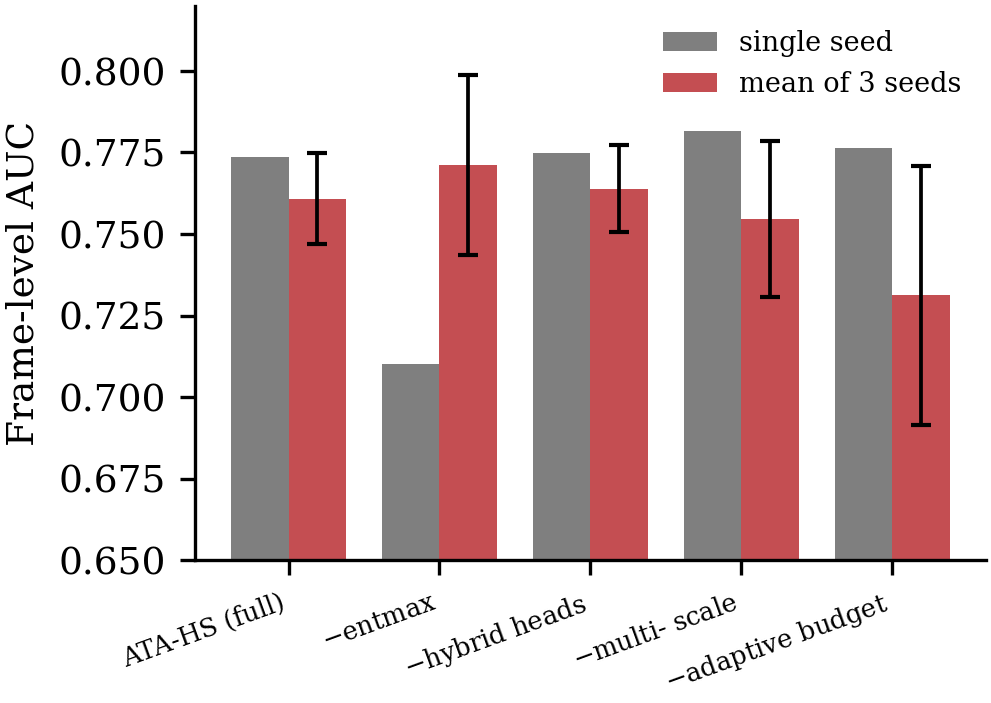
\includegraphics[width=0.6\linewidth]{figures/fig_seed_effect.png}
\caption{Single-seed versus three-seed means for the same configurations.
Conclusions drawn from one run reverse under repetition.}
\label{fig:seed}
\end{figure}

\subsection{Sampling uncertainty of the test estimate}
\label{sec:uncertainty}

Frames within a video are strongly correlated, so the effective sample size of
the test set is closer to its $290$ videos than to the $1{,}111{,}808$ frames they
contain. Resampling whole videos with replacement ($2000$ iterations) gives, for
the reproduced multiple-instance baseline under the standard protocol, a $95\%$
interval of $[0.696, 0.849]$ on frame-level AUC, a half-width of $7.6$ points.

This interval is a property of this estimate on this test set, not a constant of
the benchmark: it would differ for another model, and a larger test set would
narrow it. Its relevance is one of scale. The differences commonly reported
between methods on UCF-Crime are one to two AUC points, an order of magnitude
smaller than the sampling uncertainty of a single estimate on this test set.

\subsection{The validation signal does not predict the test metric}

Weak supervision provides only video-level labels, so model selection uses
video-level validation AUC. Over $18$ runs this quantity correlates negatively
with test frame-level AUC ($r=-0.37$, $p=0.13$; Figure~\ref{fig:valtest}).
Selecting the checkpoint with the highest validation score yields a test AUC of
$0.727$, whereas the best run in the same set attains $0.801$.

\begin{figure}[htbp]
\centering
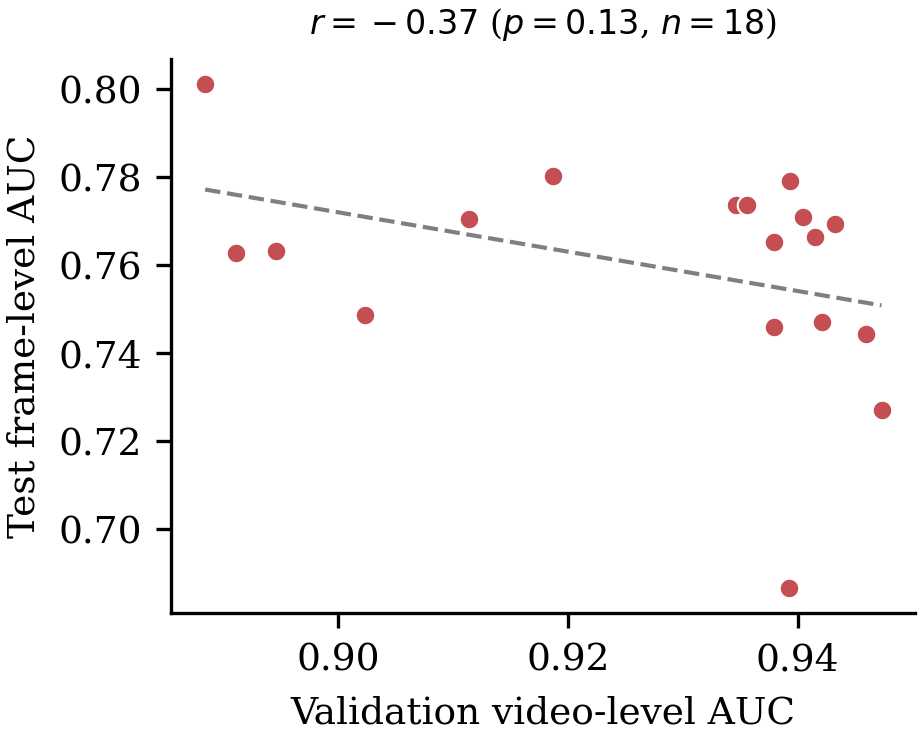
\includegraphics[width=0.48\linewidth]{figures/fig_val_vs_test.png}
\caption{Validation video-level AUC against test frame-level AUC over $18$ runs.}
\label{fig:valtest}
\end{figure}

\subsection{Localisation quality is not captured by frame-level AUC}

At a frame-level AUC of $0.769$, the temporal intersection-over-union between
thresholded predictions and annotated intervals has mean $0.098$ and median
$0.000$; only $5$ of $140$ anomalous videos exceed $0.5$. Figure~\ref{fig:qual}
shows the range: near-exact localisation, partial localisation with false
positives outside the annotated interval, complete failure, and false alarms on
normal video. Per-category results
(Figure~\ref{fig:cat}) show the spread across anomaly types, from Fighting and
Stealing above $0.93$ to Arrest at $0.64$. Figure~\ref{fig:cats} shows the
best-scoring annotated frame for each of the thirteen categories: events are
localised at high confidence in twelve, the exception being Abuse.

\begin{figure}[htbp]
\centering
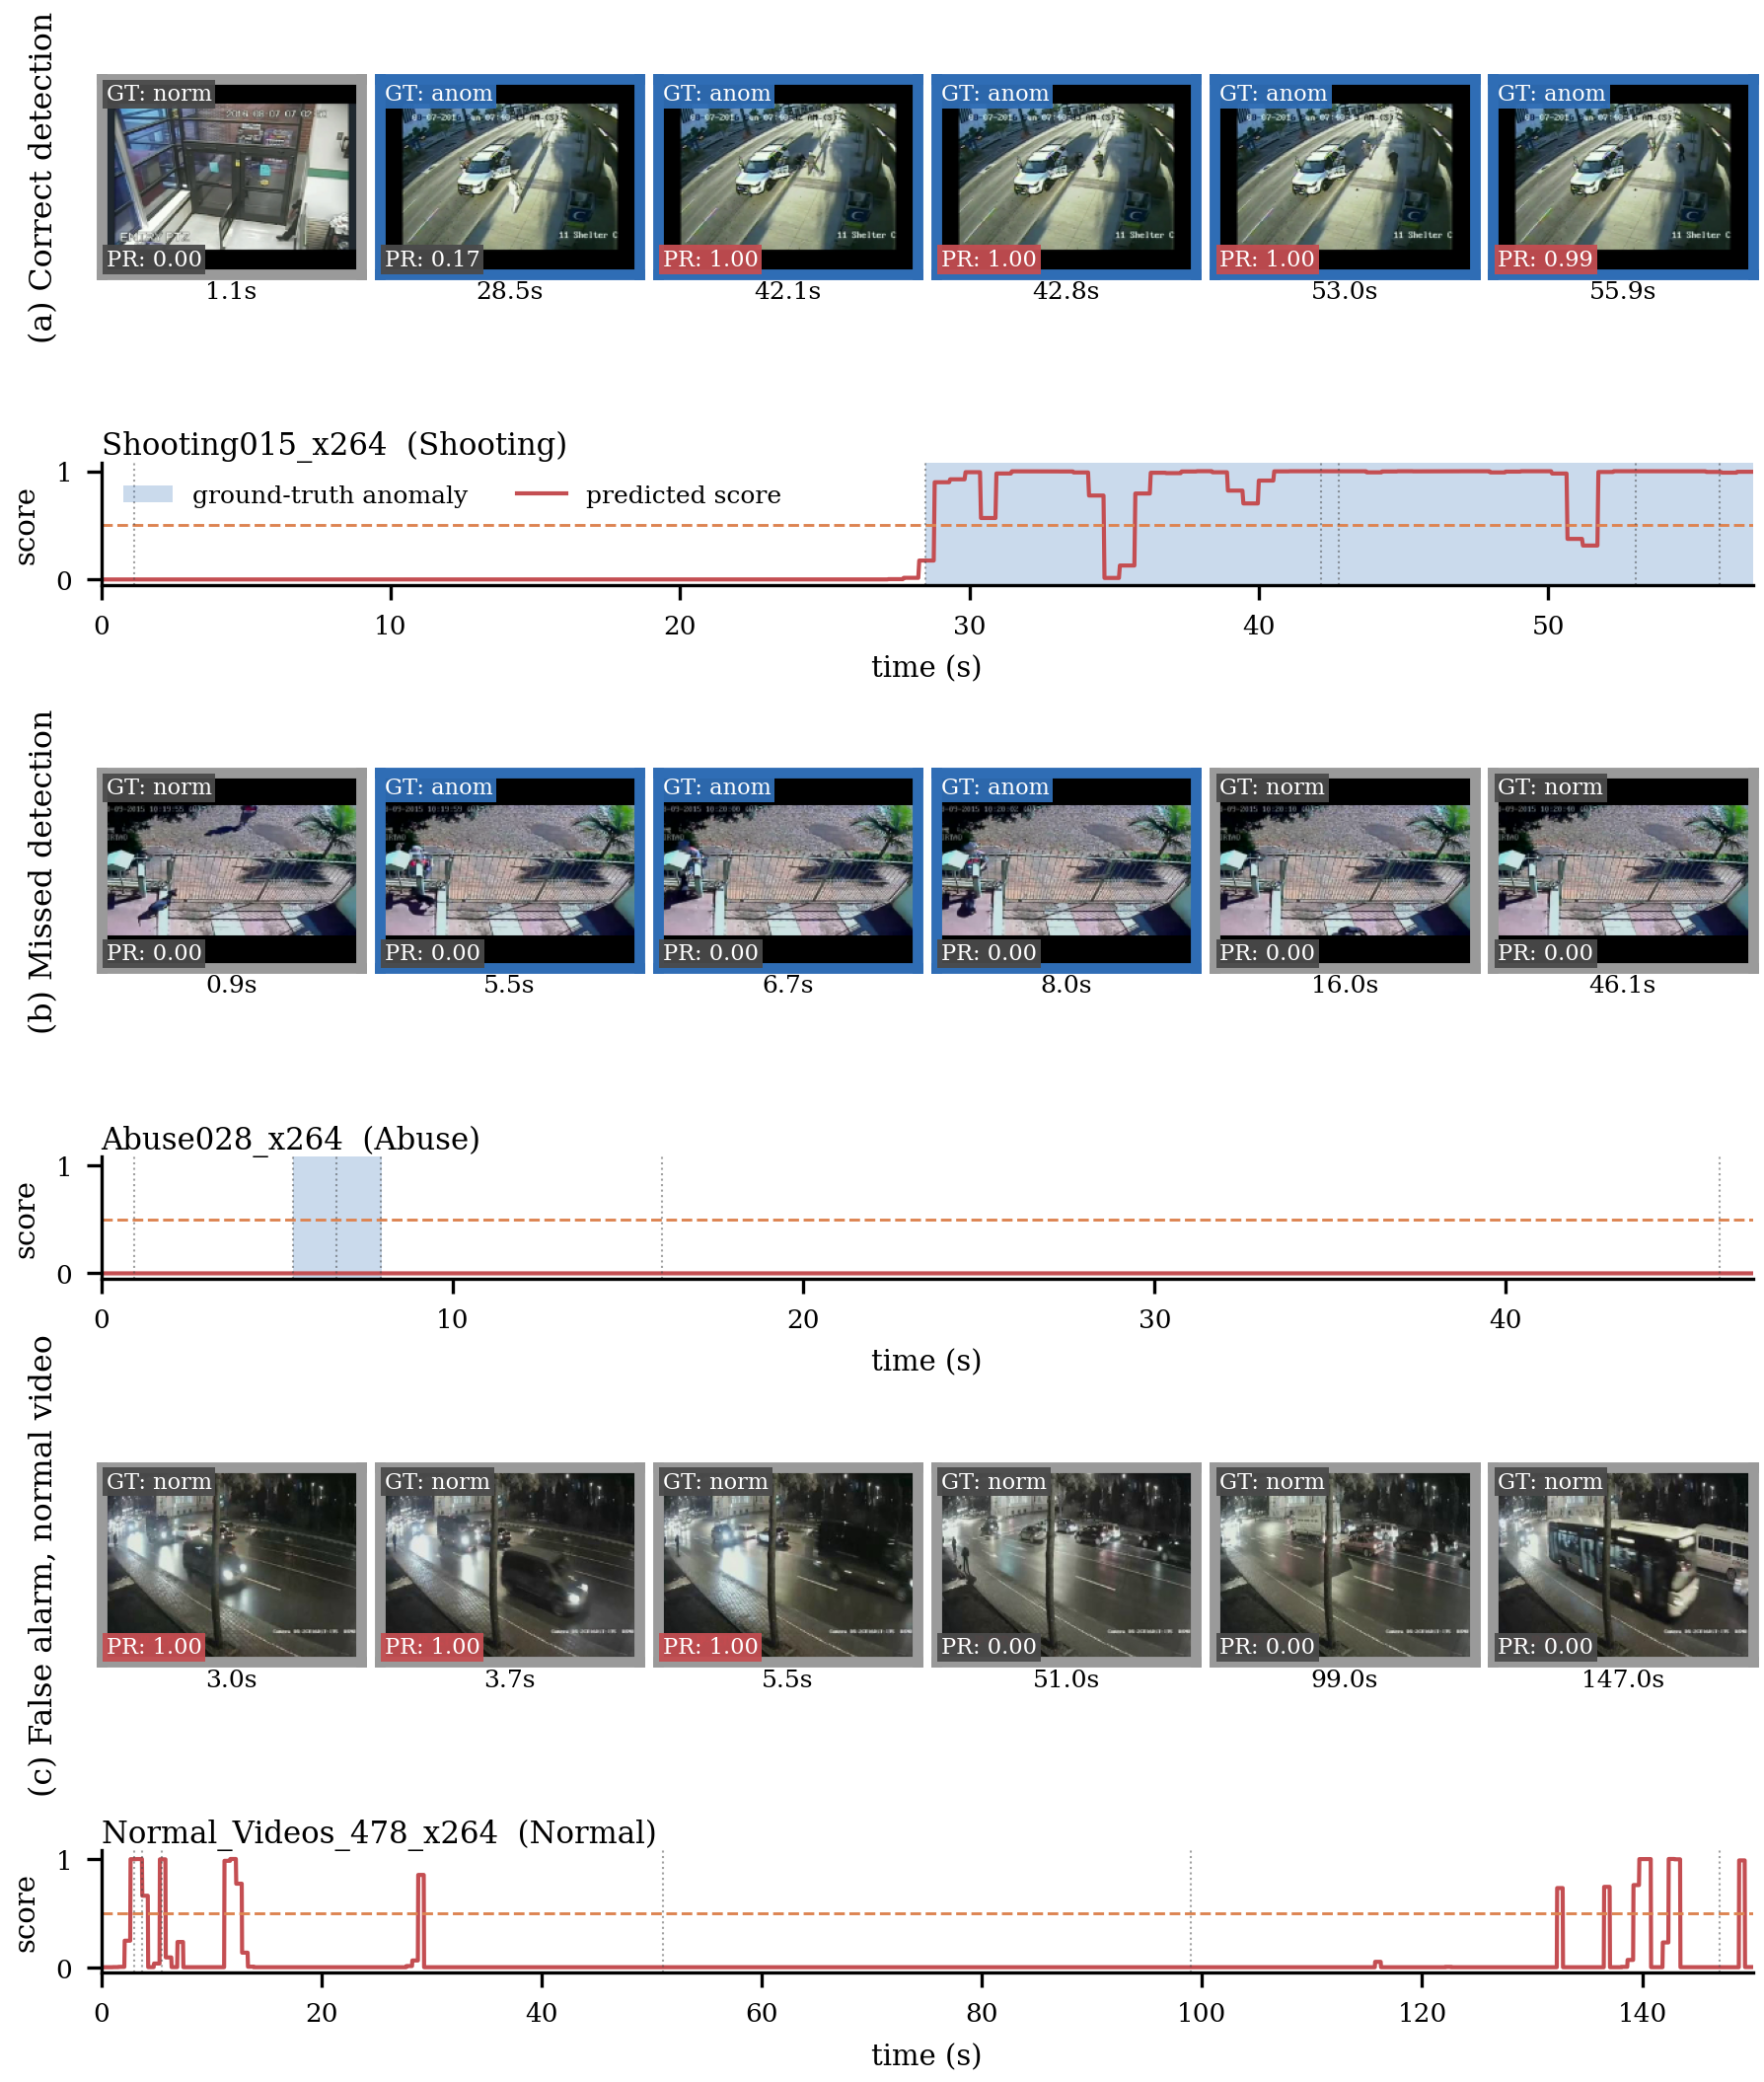
\includegraphics[width=\linewidth,height=0.88\textheight,keepaspectratio]{figures/fig_visual_results.png}
\caption{Qualitative results. Each block shows sampled frames above the score
curve for one test video. Frame border and the upper tag give the ground-truth
label (blue: annotated anomaly); the lower tag gives the predicted score (red
when above threshold). (a) Shooting015: the score rises at the interval
boundary and the annotated frames are scored $1.00$. (b) Abuse028: frames inside
the annotated interval at $5.5$--$8.0$\,s are scored $0.00$; the event is missed
entirely. (c) Normal\_Videos\_478: frames at $3.0$--$5.5$\,s are scored $1.00$
although the video contains no annotated anomaly.}
\label{fig:qual}
\end{figure}

\begin{figure}[htbp]
\centering
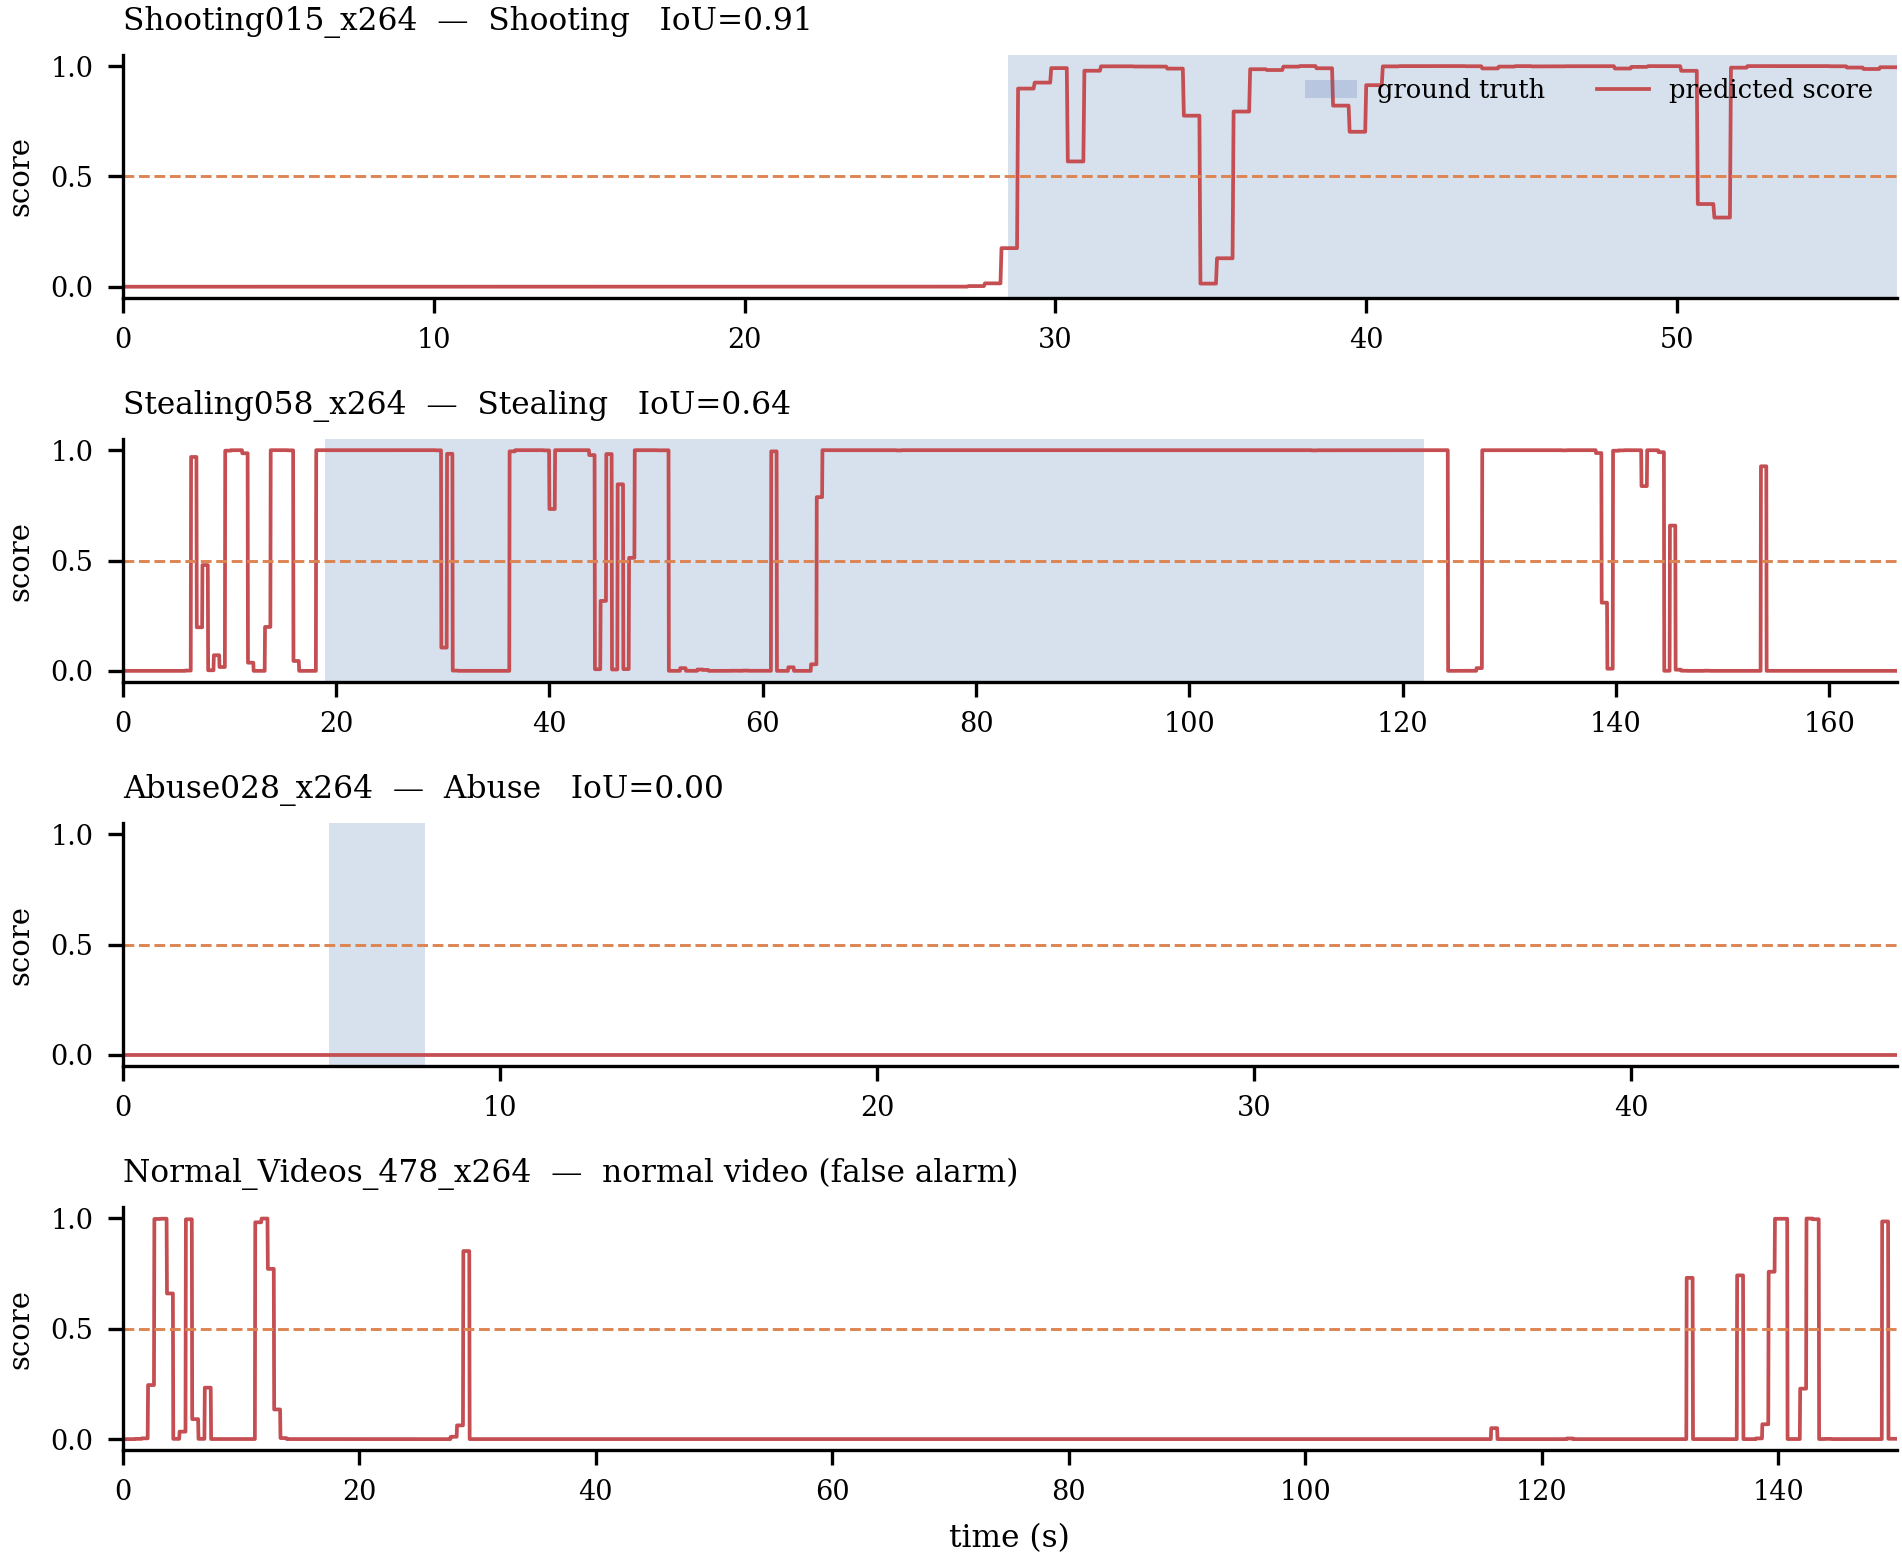
\includegraphics[width=\linewidth]{figures/fig_qualitative.png}
\caption{Predicted score against annotated intervals (shaded) for four test
videos, ordered by temporal IoU.}
\label{fig:qual2}
\end{figure}

\begin{figure}[htbp]
\centering
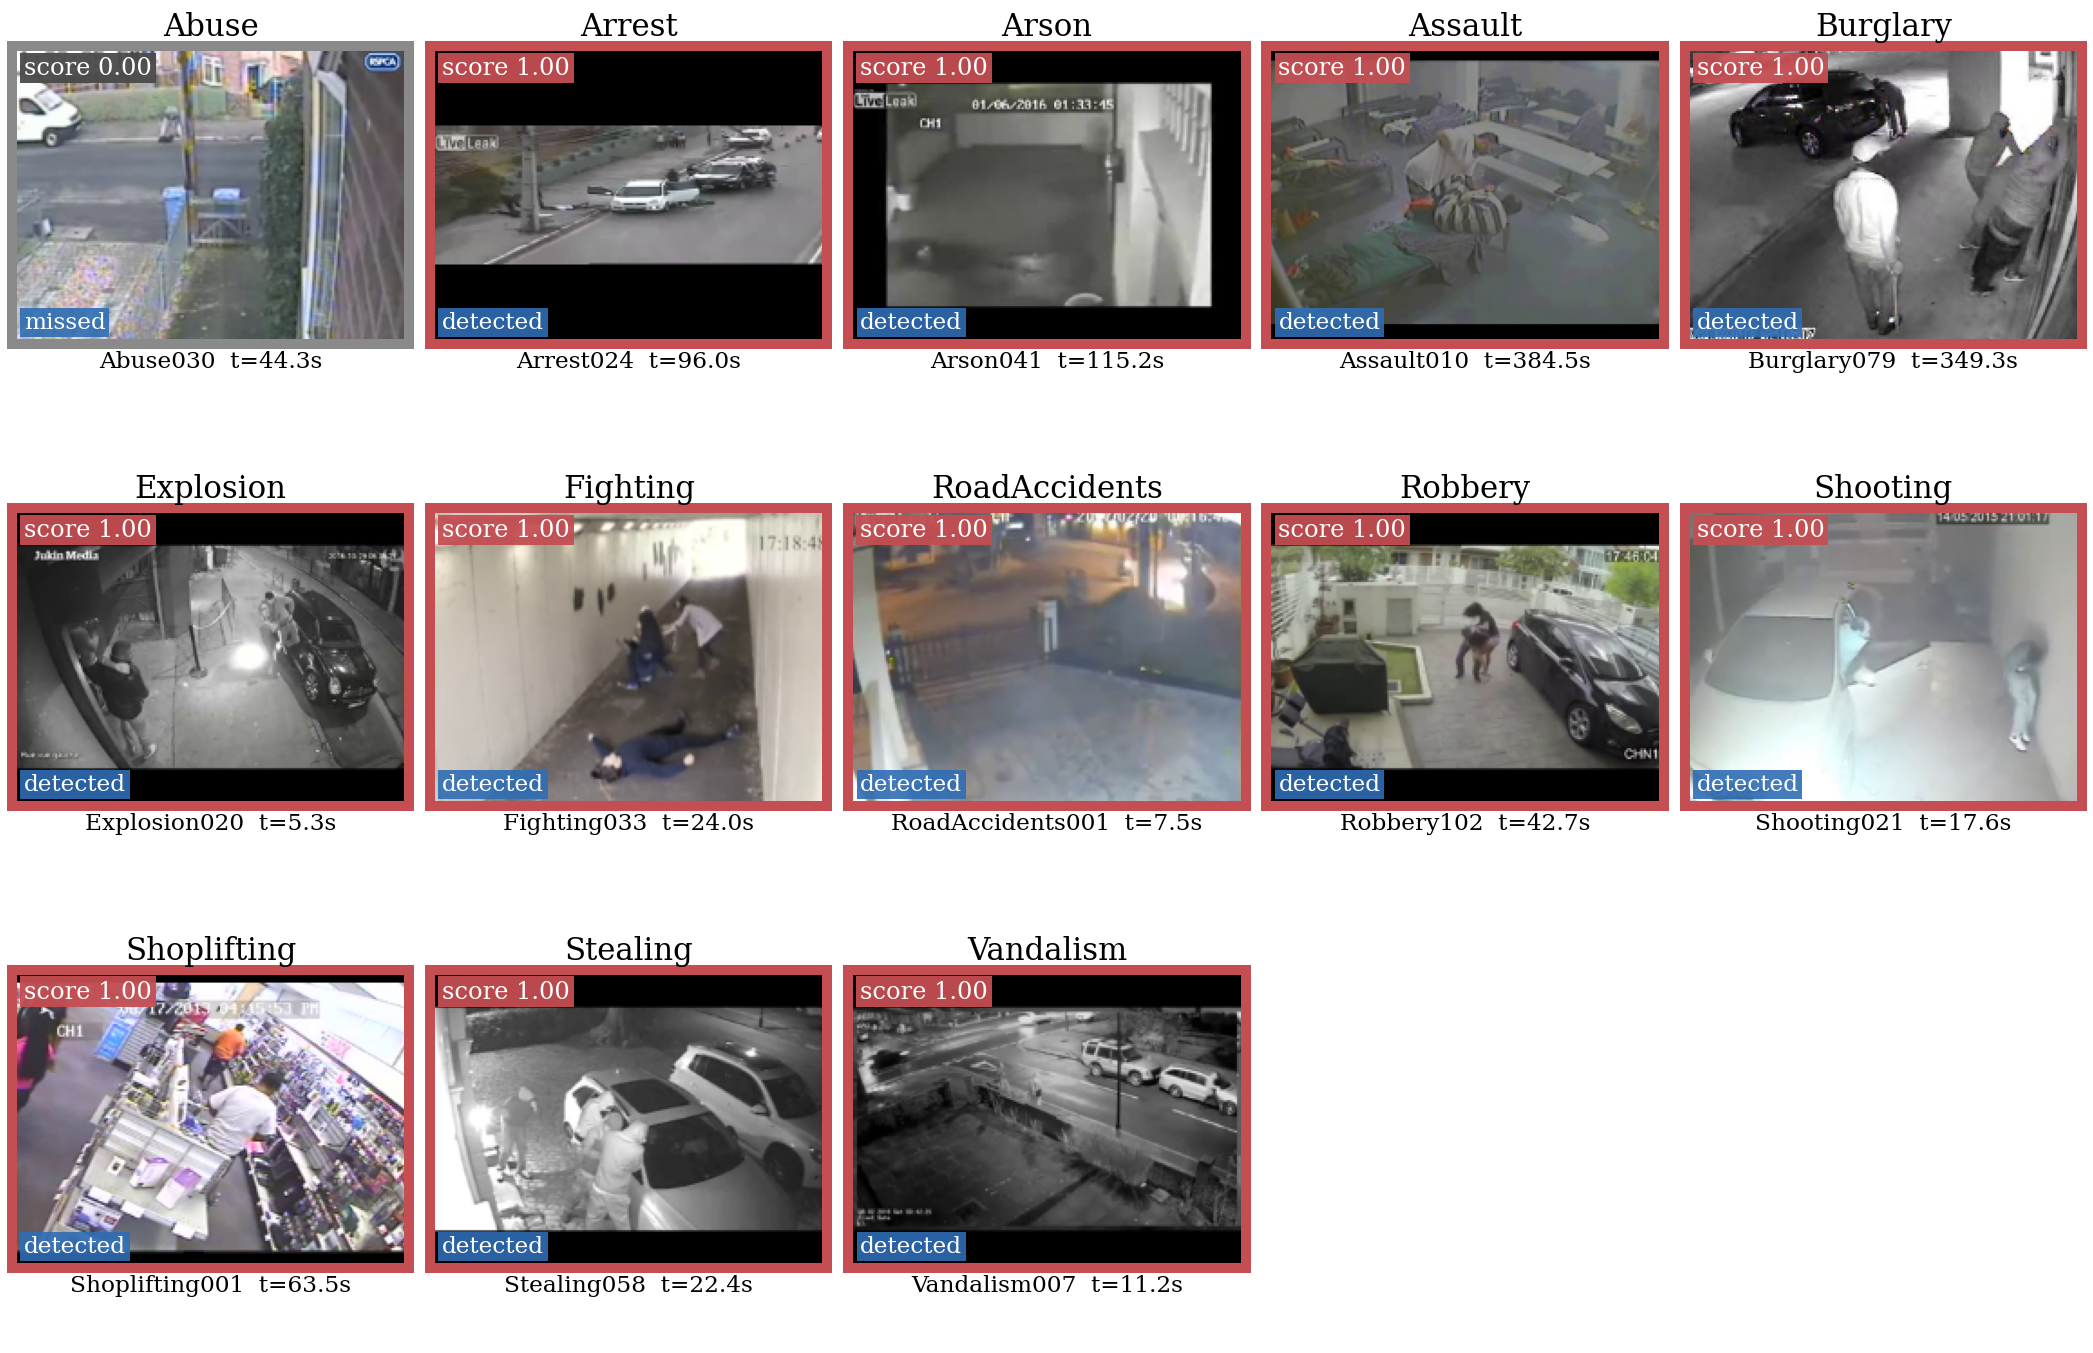
\includegraphics[width=\linewidth,height=0.88\textheight,keepaspectratio]{figures/fig_categories.png}
\caption{One example per anomaly category. For each category we show the
annotated frame that the detector scores highest, that is the best-case
detection for that category, together with its score. Red border and score tag
indicate a score above threshold. Twelve of thirteen categories contain at least
one event detected at high confidence; Abuse does not. These panels show what
the detector can localise, not how often it does so: aggregate per-category
performance is given in Figure~\ref{fig:cat} and the distribution of temporal
IoU in Section~\ref{sec:results}.}
\label{fig:cats}
\end{figure}

\begin{figure}[htbp]
\centering
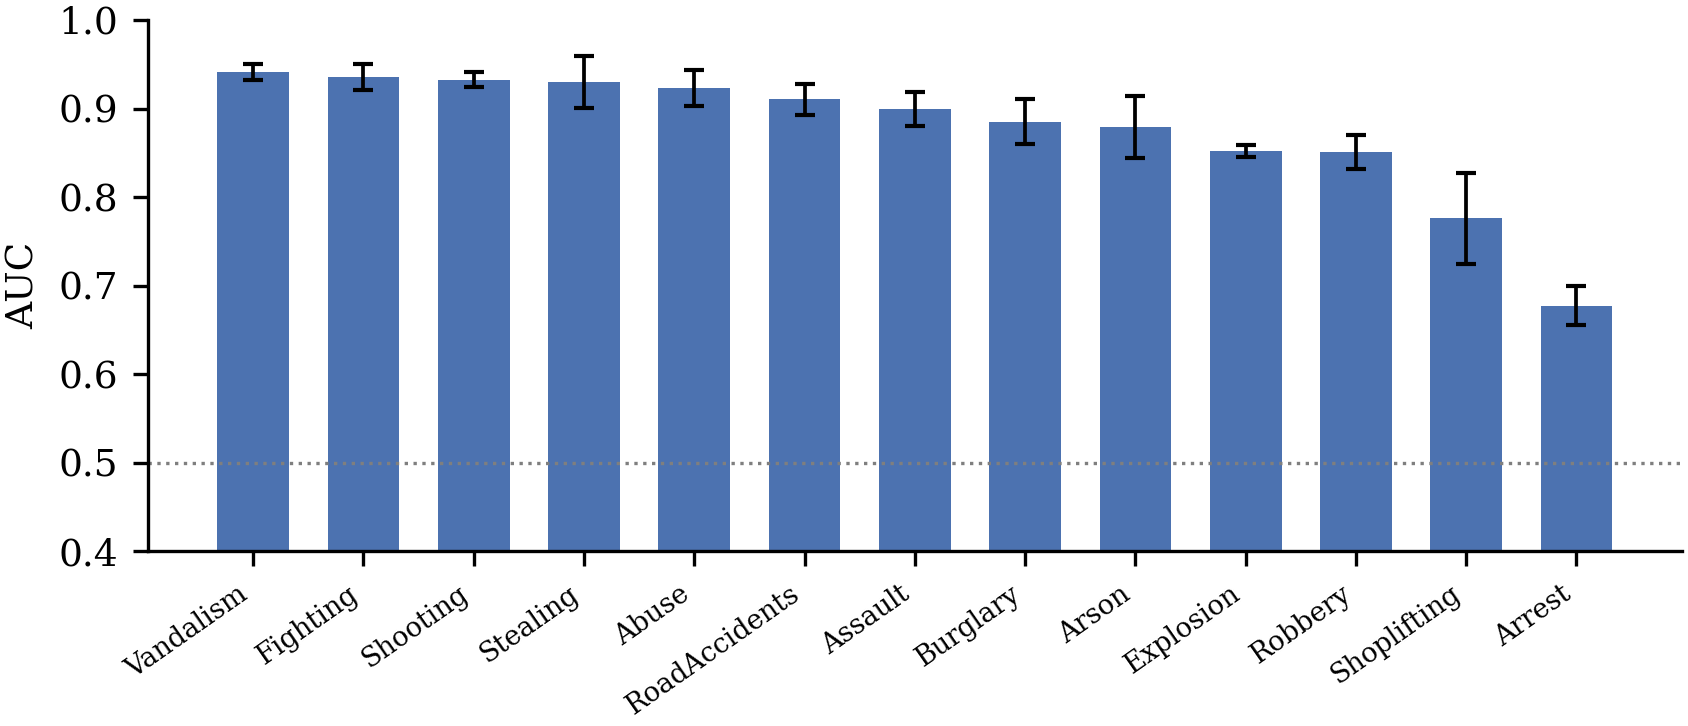
\includegraphics[width=\linewidth]{figures/fig_per_category.png}
\caption{Per-category AUC, each category pooled with all normal test videos.}
\label{fig:cat}
\end{figure}

\subsection{Masked normalisation}

Before masking the centring statistics of the deviation and temporal heads, the
model scored $0.675$; the same configuration with masked statistics scores
$0.771$. The forward pass is correct in both cases, and the defective version
attains a \emph{lower} training loss ($0.169$ versus $0.220$). A padding-invariance test is included in the released code.

% \section{Application}
% \label{sec:app}

% We release a deployed system. A Flask service holds the backbone and detector on
% the GPU; a Django REST backend manages videos, jobs and incidents; a React client
% provides upload, live camera monitoring and incident review; analysis jobs run on
% Redis-backed workers. Uploaded video is scored at $646$--$825$ frames per second,
% above $20\times$ real time, and live camera frames are scored against a rolling
% context window so the temporal model retains history. Score runs above threshold
% are stored as incidents with a thumbnail at the peak frame and a reviewer
% verdict. Each job records the threshold that produced it, so a detection can be
% traced to its settings.

\section{Discussion}
\label{sec:discussion}

\subsection{What frame-level AUC measures}

The mean-pooling row of Table~\ref{tab:comparison} has the widest consequences.
That model emits one score per video and assigns it to every frame, so it cannot
localise by construction, yet it reaches $0.775$ frame-level AUC --
indistinguishable from the multiple-instance baseline at $0.777$ and from the
proposed model at $0.761$. Ranking whole videos and localising events within them
are different capabilities, and the metric on which this benchmark is ordinarily
compared largely measures the first.

The localisation analysis gives the same conclusion from the other direction. At
$0.769$ frame-level AUC the median temporal IoU against the annotated interval is
$0.000$, and only $5$ of $140$ anomalous videos exceed $0.5$. A model can rank
frames well in aggregate while localising almost no individual event. The two
measures that do separate the methods are the AUC restricted to anomalous videos
and the fixed-threshold false-alarm rate: mean pooling scores $0.537$ and $0.304$
against $0.582$ and $0.017$ for ATA-HS. Only the first of the two survives
measurement at a matched detection rate (Section~\ref{sec:threshold}).

\subsection{What the benchmark can resolve}

For our reproduced baseline under the standard protocol, a video-level bootstrap
gives a $95\%$ interval of $[0.696, 0.849]$. This is sampling uncertainty for one
estimate on this test set rather than a fixed property of the benchmark, but its
scale matters: it is an order of magnitude larger than the one- to two-point
differences commonly reported between methods, so such differences are not
resolvable here. This applies symmetrically. No pair of methods in Table~\ref{tab:comparison} is
separated on AUC: every paired bootstrap gives $p>0.16$, and against mean pooling,
which cannot localise at all, $p=0.96$. It is why we do not claim an AUC
improvement,. The published ordering reviewed in Section~\ref{sec:related} additionally
confounds detector with representation, since substituting CLIP features raises
reported accuracy without changing the detection head; we therefore draw no
conclusion from that ordering.

Seed variance compounds the problem. The proposed model varies by $0.024$ across
seeds against $0.005$ for the baseline. A $2.66$\,M-parameter temporal model
supervised by $1610$ video-level labels is weakly constrained, whereas the
baseline scores each snippet independently through a $1.07$\,M-parameter network
and has less capacity to fit seed-specific structure. Because the ranking of
ablations reverses between one and three runs, single-run ablation on this
benchmark is not reliable at the magnitude of the effects being claimed.

Model selection is affected from a third direction. The validation signal
available under weak supervision asks whether a video contains an anomaly; the
test metric asks which frames are anomalous. Performance on one does not transfer
to the other, and over $18$ runs the two correlate at $r=-0.37$.

\subsection{Where the proposed model does differ}

At accuracy parity, ATA-HS lowers the false-alarm rate at threshold $0.5$ from
$0.023$ for the baseline and $0.028$ for dense self-attention to $0.017$, with the
smallest seed-to-seed variation of any row in Table~\ref{tab:comparison}. The
effect survives removing the multi-scale branch, the hybrid heads, the adaptive
budget and entmax individually, which attributes it to the sparse temporal
formulation rather than to any single component. Over the $150$ normal test
videos, comprising $648{,}905$ frames, the baseline raises $14{,}854$ frames above
that threshold and the full model raises $11{,}232$.

What this is, and is not, is the substance of Section~\ref{sec:threshold}. The
comparison holds the threshold fixed at $0.5$ and so assumes the two models are
comparably calibrated. They are not. Repeating it at a matched detection rate, an
operating point invariant to the score scale, reverses the ordering: the baseline
raises fewer false alarms at $95\%$ detection ($0.492$ against $0.612$) and
detects more anomalous frames at a $1\%$ false-alarm rate ($0.296$ against
$0.205$). Mean pooling, worst on FAR$_{0.5}$ by an order of magnitude, is best on
the threshold-free measure.

The sparsity budget therefore buys calibration, not discrimination. It compresses
most snippet scores toward zero, which places a large share of normal frames below
any fixed threshold and makes $0.5$ a usable default without tuning --- a real
convenience when deploying a detector, and the reason the released application
needs no per-camera threshold calibration. It does not improve the separation of
anomalous from normal frames, and we do not claim that it does. The broader point
is that FAR$_{0.5}$ has been read as a detection metric throughout this
literature while measuring detection and calibration jointly, and our own initial
reading of it was the same.

Table~\ref{tab:selection} isolates the selection mechanism. Entmax with a
predicted budget is the most accurate and the least seed-sensitive of the four,
ahead of dense attention, of entmax at a fixed temperature, and of
non-differentiable top-$K$. Its realised support is $50.6\%$ of snippets against
$100\%$ for softmax, so the sparsity is a measured property rather than one
assumed from the transformation.

The motivating account of that gate is nonetheless wrong, and
Section~\ref{sec:selection} reports the measurement that shows it. We proposed a
per-video budget because event duration varies by a factor of thirty across
categories; the predicted temperature in fact varies by four percent across the
whole test set and is uncorrelated with annotated event duration. What the gate
supplies is a schedule, dense early and sparse later, which a constant fixed at
the converged value does not reproduce: that constant scores $0.682_{\pm0.092}$
against $0.761_{\pm0.014}$. We therefore claim automatic scheduling of sparsity
rather than adaptation to content, and note that a mechanism which improves
results for reasons other than those intended is worth reporting as such.

\subsection{Secondary observations}

The masked-normalisation result is a methodological caution. Centring the
deviation and temporal heads over padded positions cost $0.096$ AUC while
\emph{lowering} the training loss. The error is a train--test inconsistency rather
than an optimisation failure: it is invisible in training diagnostics and would be
attributed to the architecture unless tested for directly.

Two properties of the split explain much of the category head's uneven per-class
recall. The training and test category balances differ
(Figure~\ref{fig:dataset}a), so the categories with the most training data are the
least tested; and several labels encode intent rather than appearance, which is
not separable from surveillance imagery alone. Robbery, Stealing and Burglary
differ in what the actor intends, not in what the camera records. At $0.379$ top-1
accuracy over $13$ classes the output is a ranking rather than a label, and the
released application presents a ranked shortlist with probabilities.

The magnitude-selection row of Table~\ref{tab:comparison} is the weakest and least
stable. We attribute this to our simplification rather than to the published
method, and note it as a limitation of the comparison rather than a finding about
RTFM.

\subsection{Recommendations}

Four practices follow for work on this benchmark. Report seed variance: in our
experiments the ranking of ablations reverses between one and three runs, and
again between three and five. Test the mechanism a component is claimed to
implement, not only whether the component helps; ours helped for a different
reason than proposed, which only direct measurement revealed. Do not select models on
video-level validation AUC, which does not predict the test metric. Report
frame-level AUC alongside a localisation measure, since AUC near $0.77$ is
attainable with no localisation at all, and report false alarms at a matched
detection rate rather than at a fixed threshold: the fixed-threshold rate moves
with the scale of a model's scores, and in our table it ranks the methods in
almost the reverse of the threshold-free order.

\paragraph{Limitations.} Experiments use a single dataset, one backbone, and
five seeds for the two models compared most closely and three for the remainder. The interval we report is specific to UCF-Crime's $290$-video test set;
larger test sets would narrow it. We did not evaluate vision-language features,
which account for most recent reported gains. Confirming that the interval is a
property of test-set size rather than of UCF-Crime specifically would require
repeating the analysis on a larger benchmark such as
XD-Violence~\citep{wu2020not}, which contains $4754$ videos.

\section{Conclusion}

We presented ATA-HS, a weakly-supervised video anomaly detector using
differentiable sparse temporal attention with a per-video sparsity budget,
together with an analysis of what the UCF-Crime benchmark can measure. ATA-HS
reaches frame-level AUC a paired bootstrap cannot separate from a
multiple-instance baseline, and lowers the false-alarm rate at the conventional
fixed threshold from $0.023$ to $0.017$. We show that this last advantage is a
property of the model's score scale rather than of its detection: at a matched
detection rate the ordering reverses, and the method with the worst
fixed-threshold rate has the best threshold-free one. The measurement analysis establishes that the benchmark's
video-level confidence interval is $\pm7.6$ AUC points, that the validation signal
available under weak supervision does not predict the test metric, and that
frame-level AUC does not reflect temporal localisation. Code, trained model and application are
released.


\appendix
\section{Anomaly category classification}
\label{app:category}

The detector answers whether an interval is anomalous, not of what kind. We
additionally train a category head on the $810$ anomalous training videos, which
carry a video-level category label. Snippet features are pooled by attention
rather than averaged, since the annotated event occupies a median $14\%$ of its
video, and the pooled descriptor is classified over the $13$ categories.

Over the $140$ anomalous test videos the head reaches $0.379$ top-1 and $0.629$
top-3 accuracy against a chance rate of $0.077$. Per-class recall is uneven:
RoadAccidents $0.74$ and Arson $0.56$, against Shooting $0.13$ and Abuse, Arrest
and Assault at $0.00$. 
\bibliographystyle{plainnat}
\bibliography{refs}

\end{document}
